% install.tex -- the TFR Installation Guide: installing a release of the
% TFR/911H software and booting NitrOS-9 Level 2 from a FujiNet.  Its
% release is \release, below.
%
% Set as the TFR Manual and Reference is (manual.tex), in the manner of
% Digital Equipment Corporation's ULTRIX documents of the early 1990s;
% its cover, in the manner of a manual of the 1970s.
%
% Build:  make -C .. install-guide     (or: xelatex install.tex, twice)

\documentclass[10pt,twoside,openany]{book}
\usepackage[letterpaper,top=0.85in,bottom=0.9in,inner=1.05in,outer=0.95in,
            headheight=14pt,headsep=0.3in,footskip=0.45in]{geometry}
\usepackage{fontspec}
\setmainfont{Times}
\setsansfont{Helvetica}[Scale=0.92]
\setmonofont{Courier}[Scale=0.95]
\usepackage{fancyhdr}
\usepackage{xcolor}
\usepackage{array,tabularx,longtable,booktabs}
\usepackage{alltt}
\usepackage{tikz}
\usetikzlibrary{calc,positioning,arrows.meta,shapes.symbols,shapes.misc,
                decorations.pathreplacing,fit,backgrounds,patterns}
\usepackage{caption}
\usepackage{float}

% The release this guide goes with: change it, and add a line to the
% revision history on the copyright page, with each release.
\newcommand{\release}{jamesBrown1}
\newcommand{\docdate}{20 October 2026}

\PassOptionsToPackage{hyphens}{url}
\usepackage[hidelinks,pdftitle={TFR Installation Guide, Release \release},
            pdfauthor={The TFR/9 Project}]{hyperref}

\setlength{\parindent}{0pt}
\setlength{\parskip}{0.7ex plus 0.2ex}
\renewcommand{\arraystretch}{1.15}
\raggedbottom
\setlength{\emergencystretch}{2em}

% ── Little helpers ─────────────────────────────────────────────────
\newcommand{\cmd}[1]{\textbf{#1}}            % a command name
\newcommand{\var}[1]{\textit{#1}}            % something you supply
\newcommand{\file}[1]{\texttt{#1}}           % a path, address, register
\newcommand{\key}[1]{\textsf{\small #1}}     % a key or button: \key{Ctrl/C}
\newcommand{\rp}[2]{\textbf{#1}(#2)}         % a reference page
\newcommand{\type}[1]{\texttt{\textbf{#1}}}  % what you type, in text
\newcommand{\sans}[1]{\textsf{#1}}
\newcommand{\pin}[1]{\textsf{#1}}            % a pin: \pin{J3-9}
\newcommand{\bs}{\textbackslash}            % a backslash, in examples
\newcommand{\lfile}[1]{\nolinkurl{#1}}      % a long path, which may break

% Examples: alltt, small Courier; \textbf for what you type.
\newenvironment{ex}{\par\vspace{0.3ex}\small\begin{alltt}}{\end{alltt}\vspace{0.3ex}}
\newenvironment{exsmall}{\par\vspace{0.3ex}\scriptsize\begin{alltt}}{\end{alltt}\vspace{0.3ex}}

% Numbered steps, as DEC wrote procedures.
\newenvironment{steps}{\begin{enumerate}\setlength{\itemsep}{0.6ex}%
  \renewcommand{\labelenumi}{\sffamily\bfseries\arabic{enumi}.}}{\end{enumerate}}

% Notes, cautions, and warnings: a word hung in the margin, between rules.
\newcommand{\notice}[2]{\par\vspace{0.8ex}\noindent
  \begin{tabularx}{\linewidth}{@{}>{\sffamily\bfseries}p{0.85in}X@{}}
  \toprule #1 & #2\\ \bottomrule\end{tabularx}\par\vspace{0.6ex}}
\newcommand{\note}[1]{\notice{Note}{#1}}
\newcommand{\caution}[1]{\notice{Caution}{#1}}

% Figures and tables, numbered by chapter as DEC numbered them: 2-1.
\captionsetup{font={small,sf},labelfont=bf,labelsep=quad,
  justification=raggedright,singlelinecheck=false}
\captionsetup[table]{position=top,skip=4pt}
\renewcommand{\thefigure}{\thechapter--\arabic{figure}}
\renewcommand{\thetable}{\thechapter--\arabic{table}}

% ── Running heads and feet ─────────────────────────────────────────
\newcommand{\thesectname}{}
\pagestyle{fancy}
\fancyhf{}
\renewcommand{\headrulewidth}{0pt}
\fancyhead[LE,RO]{\sffamily\bfseries\small Release \release}
\fancyfoot[LE,RO]{\sffamily\small\thepage}
\fancyfoot[RE,LO]{\sffamily\small\thesectname}
\fancypagestyle{plain}{\fancyhf{}\fancyfoot[LE,RO]{\sffamily\small\thepage}
  \fancyfoot[RE,LO]{\sffamily\small\thesectname}}

% Pages numbered chapter-page, as DEC numbered them: 1-1, 1-2, ... A-1.
\makeatletter
\newcommand{\chapterpages}{%
  \renewcommand{\thepage}{\thechapter--\arabic{page}}\setcounter{page}{1}}

% Chapter openings: a rule, the number big at the right, the title.
\renewcommand{\@makechapterhead}[1]{%
  \vspace*{0.4in}%
  {\color{black!75}\hrule height 2pt}\vspace{6pt}%
  \noindent\begin{minipage}[b]{0.78\textwidth}\raggedright
    \sffamily\bfseries\fontsize{24}{28}\selectfont #1\end{minipage}%
  \hfill{\sffamily\bfseries\fontsize{48}{48}\selectfont\color{black!70}\thechapter}\par
  \vspace{4pt}\hrule height 0.5pt\vspace{0.45in}}
\renewcommand{\@makeschapterhead}[1]{%
  \vspace*{0.4in}{\color{black!75}\hrule height 2pt}\vspace{6pt}%
  \noindent{\sffamily\bfseries\fontsize{24}{28}\selectfont #1}\par
  \vspace{4pt}\hrule height 0.5pt\vspace{0.45in}}

% Headings within chapters: Helvetica, numbered like 1.2.
\renewcommand{\section}{\@startsection{section}{1}{0pt}{3.2ex plus 1ex}{1.2ex}%
  {\sffamily\bfseries\large}}
\renewcommand{\subsection}{\@startsection{subsection}{2}{0pt}{2.4ex plus 0.6ex}{0.8ex}%
  {\sffamily\bfseries\normalsize}}
\setcounter{secnumdepth}{2}

% The table of contents, in Helvetica.
\renewcommand{\@pnumwidth}{2.8em}
\renewcommand{\@tocrmarg}{3.6em}
\renewcommand*{\l@chapter}[2]{\addpenalty{-\@highpenalty}\vskip 1.1em plus 1pt
  {\setlength{\@tempdima}{2em}\parindent\z@ \rightskip\@pnumwidth
   \parfillskip -\@pnumwidth \leavevmode\sffamily\bfseries
   \advance\leftskip\@tempdima \hskip -\leftskip #1\nobreak\hfil
   \nobreak\hb@xt@\@pnumwidth{\hss #2}\par}\vskip 0.3em}
\renewcommand{\l@section}{\@dottedtocline{1}{1.5em}{2.6em}}
\renewcommand{\l@subsection}{\@dottedtocline{2}{4.1em}{3.2em}}
\renewcommand*{\l@figure}{\@dottedtocline{1}{0em}{3.4em}}
\let\l@table\l@figure
\makeatother

% Two-column tables of keys or terms.
\newenvironment{keys}[1][1.1in]{\par\tabularx{\linewidth}[t]{@{}>{\raggedright\arraybackslash}p{#1}>{\raggedright\arraybackslash}X@{}}}%
  {\endtabularx\par}

% ── The diagrams ───────────────────────────────────────────────────
% Line drawings in black and grays, as the manuals had them; color only
% for wires, whose color is worth telling apart.
\definecolor{wiretx}{RGB}{222,150,0}     % yellow-orange: TFR/911H to FujiNet
\definecolor{wirerx}{RGB}{30,140,60}     % green: FujiNet to TFR/911H
\definecolor{wiregnd}{RGB}{30,30,30}     % black: ground
\definecolor{wiresd}{RGB}{50,90,170}     % blue: the SD card
\definecolor{wirepwr}{RGB}{190,40,40}    % red: power
\tikzset{
  box/.style={draw, thick, fill=black!6, rounded corners=2pt, align=center},
  lab/.style={font=\sffamily\scriptsize, align=center},
  arr/.style={-{Stealth[length=5pt]}, thick},
  callout/.style={circle, draw, thick, fill=white, inner sep=1pt,
    minimum size=13pt, font=\sffamily\bfseries\scriptsize},
}

% ── The cover ──────────────────────────────────────────────────────
% A companion to the Manual and Reference: the same cream stock, Futura,
% and stepped band of stripes, but in the harvest inks of a kitchen of
% 1974, and turning the other way.
\newfontfamily\coverfont{Futura}[UprightFont={* Medium}, BoldFont={* Bold}]
\newfontfamily\coverheavy{Futura Condensed ExtraBold}
\definecolor{cream}{RGB}{243,234,211}
\definecolor{colive}{RGB}{58,66,34}
\definecolor{cavocado}{RGB}{110,124,44}
\definecolor{charvest}{RGB}{209,160,40}
\definecolor{corange}{RGB}{214,118,36}
\definecolor{crust}{RGB}{170,64,30}
\newcommand{\coverart}{%
  \coordinate (O) at (current page.north west);
  \fill[cream] (current page.south west) rectangle (current page.north east);
  % the band: five stripes, each turning on the same centres
  \foreach \d/\c in {0.56/colive, 0.28/cavocado, 0/charvest, -0.28/corange, -0.56/crust} {
    \pgfmathsetmacro\ra{1.5+\d}
    \pgfmathsetmacro\rb{1.5-\d}
    \draw[\c, line width=0.29in, line cap=butt]
      ($(O)+(8.7,-4.85+\d)$) -- ($(O)+(3.45-\d+\ra,-4.85+\d)$)
      arc[start angle=90, end angle=180, radius=\ra]
      -- ($(O)+(3.45-\d,-8.05+\d+\rb)$)
      arc[start angle=0, end angle=-90, radius=\rb]
      -- ($(O)+(-0.3,-8.05+\d)$);
  }
  % the title
  \node[anchor=north west, inner sep=0, text=colive,
    font=\coverheavy\fontsize{168}{168}\selectfont] at ($(O)+(0.78,-0.7)$) {TFR};
  \node[anchor=north west, inner sep=0, text=colive,
    font=\coverfont\fontsize{30}{30}\selectfont] at ($(O)+(0.86,-2.72)$)
    {Installation Guide};
  \node[anchor=north west, inner sep=0, text=crust,
    font=\coverfont\fontsize{13}{13}\selectfont] at ($(O)+(0.88,-3.3)$)
    {Booting the TFR/911H from a FujiNet};
  % the release, in the open water at the right
  \node[anchor=north east, inner sep=0, text=crust, align=right,
    font=\coverfont\fontsize{11}{13}\selectfont] at ($(O)+(7.65,-6.05)$)
    {Release};
  \node[anchor=north east, inner sep=0, text=colive,
    font=\coverfont\bfseries\fontsize{26}{28}\selectfont] at ($(O)+(7.65,-6.32)$)
    {\release};
  % the foot: the order number, and who
  \draw[colive, line width=1.2pt] ($(O)+(0.85,-9.62)$) -- ($(O)+(7.65,-9.62)$);
  \node[anchor=north west, inner sep=0, text=colive, align=left,
    font=\coverfont\fontsize{9.5}{12}\selectfont] at ($(O)+(0.85,-9.78)$)
    {Order No.\ TFR-911H-IG\\Release \release, October 2026};
  \node[anchor=north east, inner sep=0, text=colive,
    font=\coverfont\bfseries\fontsize{15}{15}\selectfont] at ($(O)+(7.65,-9.8)$)
    {the tfr/9 project};
}

\begin{document}
\frontmatter
\pagestyle{empty}

% ── Title page ─────────────────────────────────────────────────────
\begin{titlepage}
\noindent\begin{tikzpicture}[remember picture, overlay, x=1in, y=1in]
  \coverart
\end{tikzpicture}
\end{titlepage}

% ── Copyright page ─────────────────────────────────────────────────
\clearpage
{\sffamily\bfseries\Large TFR Installation Guide\par}
\vspace{2pt}
{\sffamily Booting the TFR/911H from a FujiNet: Release \release\par}
\vspace{0.15in}
\begin{minipage}{0.72\textwidth}
This guide tells how to install release \release{} of the TFR/911H
software: how to flash the FujiNet's firmware with FujiNet-Flasher, make
its SD card, flash the TFR/911H's firmware, install the tether, wire the two
boards together, and boot NitrOS-9 Level 2 from the FujiNet.
\end{minipage}\par\vspace{0.6ex}

\vspace{0.2in}
{\sffamily
\begin{tabular}{@{}l l@{}}
\bfseries Order Number: & TFR-911H-IG\\[3pt]
\bfseries Release: & \release, \docdate\\[3pt]
\bfseries Revision/Update Information: & This is a new guide.\\[3pt]
\bfseries Operating System and Version: & NitrOS-9/6809 Level 2 V3.3.0\\[3pt]
\bfseries Firmware: & TFR/911H firmware v4; FujiNet firmware v1.6.2-dev (dca3ee4a3)\\[3pt]
\bfseries Hardware: & TFR/911H; an ESP32 DevKitC with 8~MB of flash and PSRAM\\
\end{tabular}\par}
\vspace*{\fill}
{\small
\textbf{TFR Installation Guide, Release \release, \docdate}

\textbf{Revision history}\\[2pt]
\begin{tabular}{@{}l l p{3.9in}@{}}
\release & 20 Oct 2026 & First printing.\\
\end{tabular}

The information in this document is subject to change without notice and
should not be construed as a commitment by anyone in particular. The
software described in this document is furnished as source code and as
binaries built from it, and may be used, copied, and changed under the
terms of the licenses that come with it: the TFR/9 software under the MIT
License; the FujiNet firmware and the FujiNet programs under the GNU
General Public License, version~3. Appendix~A tells where the source of
each part of the release is.

No responsibility is assumed for the use or reliability of software on
equipment that was soldered together at a kitchen table.

\copyright{} The TFR/9 Project contributors, 2026. All rights reserved.

\medskip
\textbf{Trademarks.} OS-9 is a trademark of Microware Systems Corporation.
NitrOS-9 is the work of the NitrOS-9 Project. Raspberry Pi is a trademark
of Raspberry Pi Ltd. ESP32 is a trademark of Espressif Systems. macOS is
a trademark of Apple Inc. Linux is a registered trademark of Linus
Torvalds. Color Computer and CoCo are associated with Tandy Corporation.
ULTRIX and DEC are trademarks of Digital Equipment Corporation.

\medskip
\textbf{About the design.} This guide is typeset as its companion, the
\emph{TFR Manual and Reference}, is: in the manner of Digital Equipment
Corporation's ULTRIX documents of the early 1990s, as a tribute, with a
cover in Futura in the manner of a manual of the 1970s. It is not a
Digital document, and it has nothing to do with Digital Equipment
Corporation or its successors.

\medskip
This document was prepared with \LaTeX{} from
\file{v4/nitros9-l2/doc/install.tex}.
}
\clearpage

\pagestyle{fancy}
\renewcommand{\thesectname}{Contents}
\setcounter{page}{3}
\tableofcontents

\clearpage
\renewcommand{\thesectname}{Figures and Tables}
{\sffamily\bfseries\large Figures\par}\vspace{1ex}
\makeatletter\@starttoc{lof}\makeatother
\vspace{3ex}
{\sffamily\bfseries\large Tables\par}\vspace{1ex}
\makeatletter\@starttoc{lot}\makeatother

% ── Preface ────────────────────────────────────────────────────────
\chapter*{About This Guide}
\addcontentsline{toc}{chapter}{About This Guide}
\renewcommand{\thesectname}{About This Guide}

This guide takes you from a bare TFR/911H and an ESP32 board to NitrOS-9
Level 2 booting from the FujiNet's SD card, with the network programs
working: the weather, the news, stock quotes, Bounce World, and Fuji
Battleship. Every file it asks for is in the release, \release.

\section*{Audience}
This guide is for anyone setting up a TFR/911H with a FujiNet: no
knowledge of OS-9, the RP2350B, or the ESP32 is assumed. You need to be
able to copy files, open a terminal window and type commands in it, and
push three jumper wires onto header pins.

\section*{Organization}
This guide has seven chapters and three appendices:

\begin{tabularx}{\linewidth}{@{}>{\bfseries}l X@{}}
Chapter 1 & What you are building, what is in the release, what you
need, and the installation at a glance.\\
Chapter 2 & Flashing the FujiNet's firmware with FujiNet-Flasher.\\
Chapter 3 & Making the FujiNet's SD card: the boot disk and the
FujiNet's settings.\\
Chapter 4 & Flashing the TFR/911H's firmware, and installing the
tether.\\
Chapter 5 & Wiring the FujiNet to the TFR/911H, and checking the link.\\
Chapter 6 & Booting NitrOS-9 from the FujiNet, and what to do next.\\
Chapter 7 & Troubleshooting.\\
Appendix A & The release: its files, their checksums, their sources, and
how it was tested.\\
Appendix B & Building the release from source.\\
Appendix C & Pins and settings, for reference.\\
\end{tabularx}

\section*{Related Documents}
\begin{itemize}\setlength{\itemsep}{0pt}
\item The \emph{TFR Manual and Reference} (TFR-911H-MR), in the release:
NitrOS-9 on the TFR/911H, its commands, the FujiNet, and how it all works.
\item \file{v4/nitros9-l2/fujinet/README.md} in the TFR/9 source, on
setting up and programming the FujiNet.
\item The FujiNet project's pages, at \file{fujinet.online}, and its wiki,
at \lfile{github.com/FujiNetWIFI/fujinet-firmware/wiki}.
\end{itemize}

\section*{Conventions}
\begin{tabularx}{\linewidth}{@{}>{\raggedright\arraybackslash}p{1.3in}X@{}}
\toprule
\textbf{Convention} & \textbf{Meaning}\\
\midrule
\texttt{\$} & A shell prompt on your computer.\\
\texttt{TCL>} & The TFR/911H firmware's prompt, before an OS boots.\\
\texttt{OS9:} & The NitrOS-9 Shell prompt.\\
\type{bold type} & In examples, what you type.\\
\var{italic} & Something you supply: a file name, a device.\\
\key{Ctrl/]} & Hold down the Ctrl key while you press \key{]}.\\
\key{FLASH} & A button on a board, by the name printed beside it.\\
\pin{J3-9} & Pin 9 of the header marked J3.\\
\pin{IO33} & A pin of the ESP32 board, by the name printed beside it:
here, GPIO~33.\\
\file{jamesBrown1/} & A file or folder of the release.\\
\bottomrule
\end{tabularx}

% ═══════════════════════════════════════════════════════════════════
\mainmatter
\chapter{Before You Start}
\chapterpages
\renewcommand{\thesectname}{Before You Start}

This chapter describes what you are building, what is in the release,
and what you need, and it lists the steps that the rest of the guide
takes one at a time.

\section{What You Are Building}

The TFR/911H is a single board computer with a Hitachi 6309 for its CPU
and a Raspberry Pi RP2350B for everything else: the 6309's clock, its
memory, and all of its I/O. The RP2350B talks USB to a program on your
computer, the \emph{tether}, which is the board's terminal.

A FujiNet is an ESP32 with WiFi and an SD card. Three wires join it to
the TFR/911H, and over them the two speak DriveWire, the protocol a Color
Computer uses to reach disks and the network. The FujiNet's SD card holds
the disk that NitrOS-9 boots from; its WiFi reaches the servers that the
network programs talk to. Figure~\ref{fig:system} shows the whole
system.

\begin{figure}[htbp]
\centering
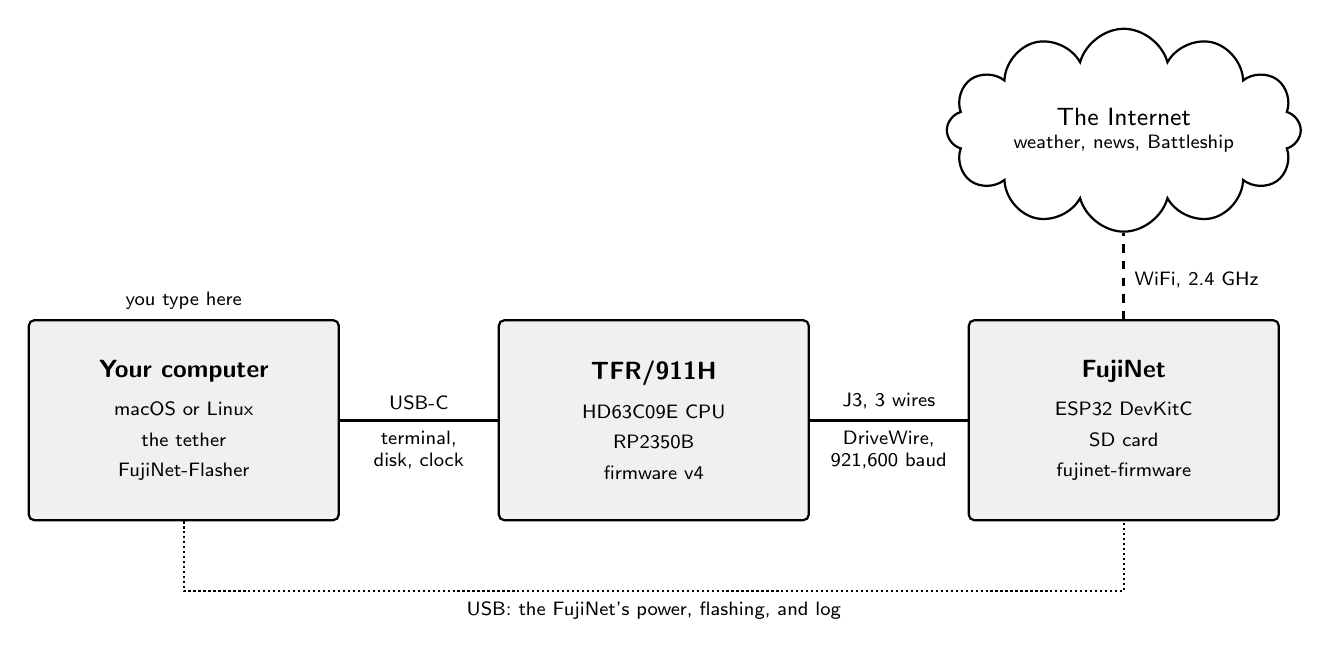
\begin{tikzpicture}[x=1in, y=1in, font=\sffamily\small]
  \node[box, minimum width=1.55in, minimum height=1.0in] (pc) at (0,0)
    {\bfseries Your computer\\[3pt]\scriptsize macOS or Linux\\\scriptsize the tether\\\scriptsize FujiNet-Flasher};
  \node[box, minimum width=1.55in, minimum height=1.0in] (tfr) at (2.35,0)
    {\bfseries TFR/911H\\[3pt]\scriptsize HD63C09E CPU\\\scriptsize RP2350B\\\scriptsize firmware v4};
  \node[box, minimum width=1.55in, minimum height=1.0in] (fn) at (4.7,0)
    {\bfseries FujiNet\\[3pt]\scriptsize ESP32 DevKitC\\\scriptsize SD card\\\scriptsize fujinet-firmware};
  \node[cloud, draw, thick, cloud puffs=12, aspect=2.4, fill=white,
    minimum width=1.7in, minimum height=0.75in, lab] (net) at (4.7,1.45)
    {\small The Internet\\weather, news, Battleship};
  \draw[very thick] (pc) -- node[lab, above]{USB-C} node[lab, below]{terminal,\\disk, clock} (tfr);
  \draw[very thick] (tfr) -- node[lab, above]{J3, 3 wires} node[lab, below]{DriveWire,\\921{,}600 baud} (fn);
  \draw[very thick, dashed] (fn) -- node[lab, right, pos=0.45]{WiFi, 2.4 GHz} (net);
  \draw[thick, densely dotted] (pc.south) -- ++(0,-0.35) -| (fn.south)
    node[lab, pos=0.25, below]{USB: the FujiNet's power, flashing, and log};
  \node[lab, anchor=south] at (pc.north) {you type here};
\end{tikzpicture}
\caption{The TFR/911H, the FujiNet, and your computer}\label{fig:system}
\end{figure}

When you are done, the TFR/911H's firmware boots NitrOS-9 Level 2 from
the file \file{level2-fn.dsk} on the FujiNet's SD card, which NitrOS-9
calls \file{/DD}, its system disk. You use it through the tether's window
on your computer.

\section{What Is in the Release}

The release is a folder, \file{jamesBrown1/}, laid out as
Figure~\ref{fig:tree} shows. Appendix~A lists every file with its size and
checksum.

\begin{figure}[htbp]
\begin{exsmall}
jamesBrown1/
  README.txt                       what this is, and the steps in brief
  TFR-Installation-Guide-jamesBrown1.pdf
                                   this guide
  TFR-Manual-and-Reference-1.3.pdf the TFR Manual and Reference
  SHA256SUMS                       a checksum for every file
  tfr911h/
    tfr911h_v4.uf2                 the TFR/911H's firmware                     (Chapter 4)
  fujinet/
    fujinet-COCO-HS-UART-v1.6.2-dev-dca3ee4a3.zip
                                   the FujiNet's firmware, for FujiNet-Flasher (Chapter 2)
  sdcard/                          what goes on the FujiNet's SD card          (Chapter 3)
    fnconfig.ini                   the FujiNet's settings: WiFi, host 1, device slot 1
    tfr911/
      level2-fn.dsk                NitrOS-9 Level 2, booting from the FujiNet
  tether/                          what stays on your computer                 (Chapter 4)
    run-tfr.sh                     starts the tether and boots NitrOS-9
    tether-darwin-arm64            the tether for a Mac with Apple silicon
    tether-darwin-amd64            ... a Mac with an Intel processor
    tether-linux-amd64             ... a Linux PC
    tether-linux-arm64             ... 64-bit Linux on ARM: a Raspberry Pi 4 or 5
    tether-linux-arm               ... 32-bit Linux on ARMv7: a Raspberry Pi 2 or 3
    level2.dsk                     the tether's own disk, /H0
  licenses/
    LICENSE-tfr9-MIT.txt           the TFR/9 software's license
    LICENSE-GPL-3.0.txt            the FujiNet firmware's and programs' license
\end{exsmall}
\caption{The release folder}\label{fig:tree}
\end{figure}

There are two disks. \file{sdcard/tfr911/level2-fn.dsk} goes on the
FujiNet's SD card and is the one NitrOS-9 boots from. \file{tether/level2.dsk}
stays on your computer, where the tether serves it as a second hard disk,
\file{/H0}; it can also boot NitrOS-9 by itself, without the FujiNet
(Section~\ref{sec:l2}). Both hold the same system and the same commands.

\section{What You Need}

\begin{table}[H]
\caption{What you need}\label{tab:need}
\begin{tabularx}{\linewidth}{@{}>{\raggedright\arraybackslash}p{1.45in}X@{}}
\toprule
\textbf{Item} & \textbf{Notes}\\
\midrule
A TFR/911H & With its HD63C09E (or 6309E) in the socket.\\
An ESP32 board for the FujiNet & An Espressif ESP32-DevKitC with an
ESP32-WROVER module, which has 8~MB of flash and PSRAM: the
ESP32-DevKitC-VE, for one. The firmware needs both the 8~MB and the PSRAM;
it will not run on a board with 4~MB of flash, or on an ESP32-WROOM
module, which has no PSRAM. A FujiNet built for the Centipede also
works.\\
An SD card, and a way to connect it & A microSD card of 32~GB or less.
If your ESP32 board has no SD card slot, a microSD breakout board for
3.3~volts and six more jumper wires (Section~\ref{sec:sd}).\\
Three jumper wires & Male at one end and female at the other, 15~cm (6
inches) long or less: the TFR/911H's header J3 is a socket, and the
DevKitC's pins are pins. Yellow, green, and black make the wiring easy to
check.\\
Two USB cables & One for the TFR/911H (USB-C), and one for the ESP32
board (usually micro-USB). Both must carry data, not only charge.\\
A computer & A Mac (macOS 11 or later, Apple silicon or Intel) or a
Linux computer (a PC, or a Raspberry Pi 2 or later), with two free USB
ports, an SD card reader, and a terminal of at least 80 columns by 24
lines that shows UTF-8. This release has no tether for Windows.\\
FujiNet-Flasher & The FujiNet project's flashing program, version 1.5.0 or
later, from \file{github.com/FujiNetWIFI/fujinet-flasher/releases}.\\
A WiFi network & 2.4~GHz, for the network programs. NitrOS-9 boots from
the SD card without it.\\
\bottomrule
\end{tabularx}
\end{table}

\section{The Installation at a Glance}

Figure~\ref{fig:steps} shows the six steps. The FujiNet comes first, so
that it is ready when the TFR/911H first asks it for something.

\begin{figure}[htbp]
\centering
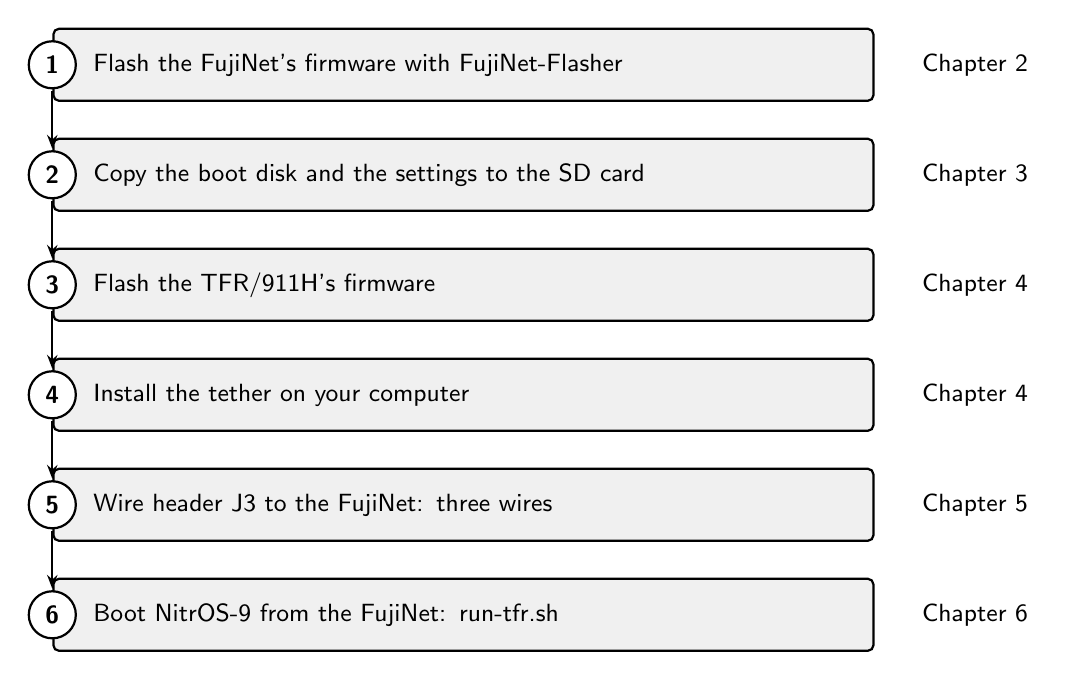
\begin{tikzpicture}[x=1in, y=1in, font=\sffamily\small]
  \foreach \n/\t/\c [count=\i] in {
    1/Flash the FujiNet's firmware with FujiNet-Flasher/Chapter 2,
    2/Copy the boot disk and the settings to the SD card/Chapter 3,
    3/{Flash the TFR/911H's firmware}/Chapter 4,
    4/Install the tether on your computer/Chapter 4,
    5/Wire header J3 to the FujiNet: three wires/Chapter 5,
    6/Boot NitrOS-9 from the FujiNet: run-tfr.sh/Chapter 6} {
    \node[box, minimum width=4.1in, minimum height=0.36in, anchor=west,
      text width=3.7in, align=left] (s\i) at (0.45,-0.55*\i) {\t};
    \node[callout, minimum size=17pt, font=\sffamily\bfseries\small]
      at (0.45,-0.55*\i) {\n};
    \node[lab, anchor=west, font=\sffamily\small] at (4.75,-0.55*\i) {\c};
  }
  \foreach \i in {1,...,5}
    \draw[arr] (0.45,-0.55*\i-0.13) -- (0.45,-0.55*\i-0.42);
\end{tikzpicture}
\caption{The installation, step by step}\label{fig:steps}
\end{figure}

% ═══════════════════════════════════════════════════════════════════
\chapter{Flashing the FujiNet}
\chapterpages
\renewcommand{\thesectname}{Flashing the FujiNet}

This chapter describes the ESP32 board the FujiNet runs on, how to give
it an SD card if it has none, and how to flash its firmware with
FujiNet-Flasher.

\section{The ESP32 Board}

The FujiNet firmware in the release, \lfile{fujinet/fujinet-COCO-HS-UART-v1.6.2-dev-dca3ee4a3.zip},
is \emph{fujinet-firmware} built for the board
\texttt{fujinet-coco-devkitc-centipede}: the Color Computer's FujiNet,
speaking DriveWire over a plain 3.3-volt serial link at a fixed 921{,}600
baud on the ESP32's UART1, which is what the TFR/911H expects. It was made
for an ESP32-DevKitC, and Figure~\ref{fig:devkitc} shows the pins it uses
on one.

\begin{figure}[htbp]
\centering
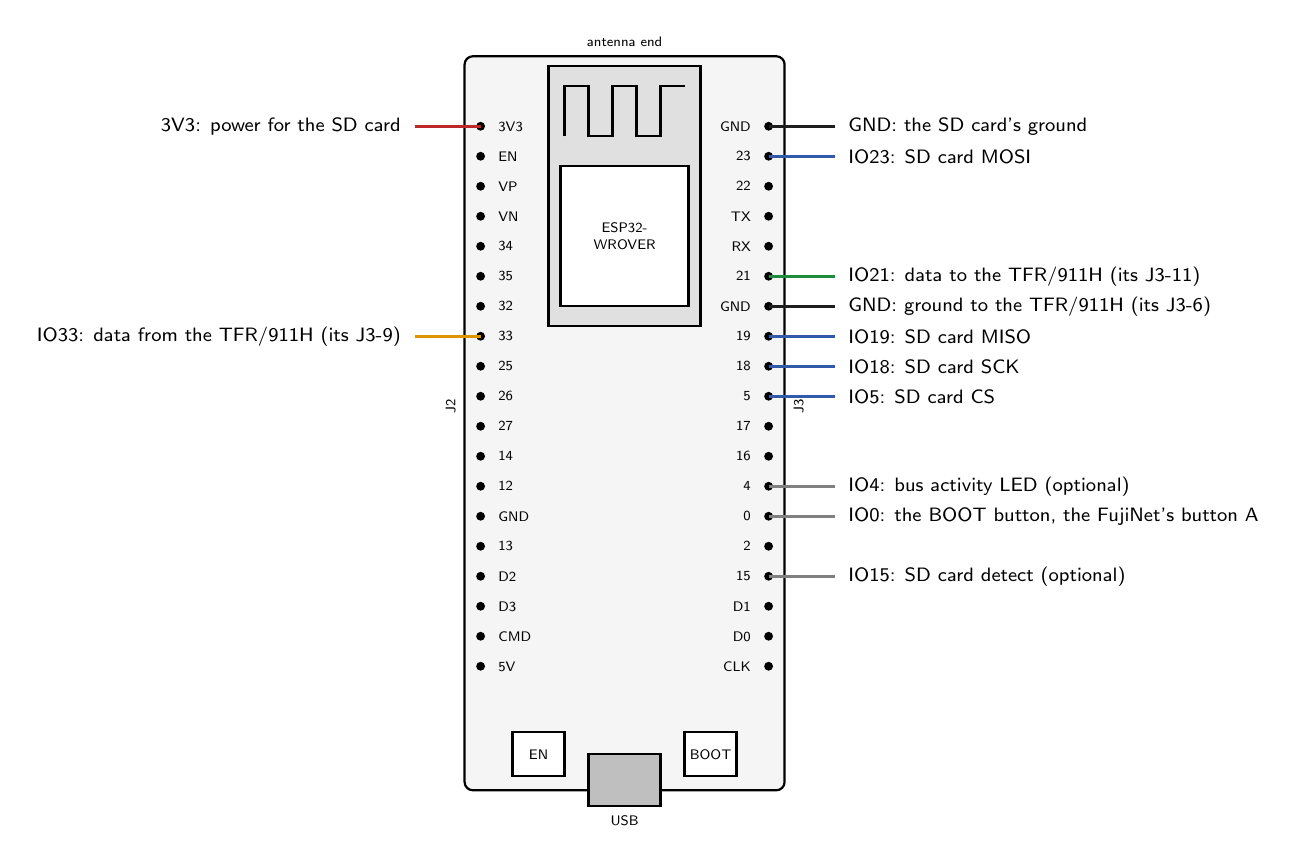
\begin{tikzpicture}[x=1in, y=1in, font=\sffamily\scriptsize]
  % the board
  \def\pitch{0.15}
  \draw[thick, fill=black!4, rounded corners=3pt] (0,-0.32) rectangle (1.6,3.35);
  % the module, with its antenna at the top
  \draw[thick, fill=black!12] (0.42,2.0) rectangle (1.18,3.3);
  \draw[thick, fill=white] (0.48,2.1) rectangle (1.12,2.8)
    node[midway, align=center, font=\sffamily\tiny]{ESP32-\\WROVER};
  \draw[thick] (0.5,2.95) -- (0.5,3.2) -- (0.62,3.2) -- (0.62,2.95) -- (0.74,2.95)
    -- (0.74,3.2) -- (0.86,3.2) -- (0.86,2.95) -- (0.98,2.95) -- (0.98,3.2) -- (1.1,3.2);
  \node[font=\sffamily\tiny] at (0.8,3.35) [above] {antenna end};
  % USB and the two buttons at the other end
  \draw[thick, fill=black!25] (0.62,-0.4) rectangle (0.98,-0.14);
  \node[font=\sffamily\tiny, below] at (0.8,-0.4) {USB};
  \draw[thick, fill=white] (0.24,-0.25) rectangle (0.5,-0.03)
    node[midway, font=\sffamily\tiny]{EN};
  \draw[thick, fill=white] (1.1,-0.25) rectangle (1.36,-0.03)
    node[midway, font=\sffamily\tiny]{BOOT};
  % the headers: J2 on the left, J3 on the right, pin 1 at the antenna end
  \foreach \l [count=\i] in {3V3,EN,VP,VN,34,35,32,33,25,26,27,14,12,GND,13,D2,D3,CMD,5V} {
    \pgfmathsetmacro\y{3.0-(\i-1)*\pitch}
    \fill (0.08,\y) circle (1.6pt);
    \node[anchor=west, font=\sffamily\tiny] at (0.12,\y) {\l};
  }
  \foreach \l [count=\i] in {GND,23,22,TX,RX,21,GND,19,18,5,17,16,4,0,2,15,D1,D0,CLK} {
    \pgfmathsetmacro\y{3.0-(\i-1)*\pitch}
    \fill (1.52,\y) circle (1.6pt);
    \node[anchor=east, font=\sffamily\tiny] at (1.48,\y) {\l};
  }
  \node[font=\sffamily\tiny, rotate=90] at (-0.07,1.6) {J2};
  \node[font=\sffamily\tiny, rotate=90] at (1.67,1.6) {J3};
  % what the FujiNet uses, on the left (J2)
  \foreach \i/\c/\t in {8/wiretx/{IO33: data from the TFR/911H (its J3-9)},
                        1/wirepwr/{3V3: power for the SD card}} {
    \pgfmathsetmacro\y{3.0-(\i-1)*\pitch}
    \draw[\c, very thick] (0.08,\y) -- (-0.25,\y);
    \node[anchor=east, align=right] at (-0.27,\y) {\t};
  }
  % and on the right (J3)
  \foreach \i/\c/\t in {1/wiregnd/{GND: the SD card's ground},
                        2/wiresd/{IO23: SD card MOSI},
                        6/wirerx/{IO21: data to the TFR/911H (its J3-11)},
                        7/wiregnd/{GND: ground to the TFR/911H (its J3-6)},
                        8/wiresd/{IO19: SD card MISO},
                        9/wiresd/{IO18: SD card SCK},
                        10/wiresd/{IO5: SD card CS},
                        13/black!50/{IO4: bus activity LED (optional)},
                        14/black!50/{IO0: the BOOT button, the FujiNet's button A},
                        16/black!50/{IO15: SD card detect (optional)}} {
    \pgfmathsetmacro\y{3.0-(\i-1)*\pitch}
    \draw[\c, very thick] (1.52,\y) -- (1.85,\y);
    \node[anchor=west] at (1.87,\y) {\t};
  }
\end{tikzpicture}
\caption{An ESP32-DevKitC, seen from above, and the pins the FujiNet uses}\label{fig:devkitc}
\end{figure}

The pins that matter most are the three that go to the TFR/911H:
\pin{IO33} (the FujiNet's receive data), \pin{IO21} (its transmit data),
and a ground. Chapter~5 wires them. The DevKitC's \key{BOOT} button is the
FujiNet's button~A; its \key{EN} button restarts the ESP32.

A DevKitC has no Safe Reset button, the FujiNet's button~C, and the
firmware in this release leaves it out. Older firmware gave the button
\pin{IO14}, which a DevKitC leaves unconnected; the floating pin picked up
the UART beside it and restarted the FujiNet every few seconds under disk
traffic. That was fixed in fujinet-firmware pull request 2034, which this
firmware includes.

\section{Adding an SD Card}\label{sec:sd}

If your ESP32 board has no SD card slot, wire a microSD breakout board to
it as Table~\ref{tab:sd} shows. Use a breakout made for 3.3~volts, or one
with its own regulator and level shifters that takes 3.3~volts in. The
card-detect wire is optional: without it, the FujiNet looks for the card
only when it starts.

\begin{table}[H]
\caption{Wiring a microSD breakout to the DevKitC}\label{tab:sd}
\begin{tabularx}{\linewidth}{@{}l l l X@{}}
\toprule
\textbf{Breakout} & \textbf{DevKitC pin} & \textbf{Header} & \textbf{Signal}\\
\midrule
CS & \pin{IO5} & \pin{J3-10} & Chip select\\
SCK (CLK) & \pin{IO18} & \pin{J3-9} & Clock\\
MOSI (DI) & \pin{IO23} & \pin{J3-2} & Data to the card\\
MISO (DO) & \pin{IO19} & \pin{J3-8} & Data from the card\\
VCC (3V3) & \pin{3V3} & \pin{J2-1} & Power\\
GND & \pin{GND} & \pin{J3-1} & Ground\\
CD & \pin{IO15} & \pin{J3-16} & Card detect, if the breakout has it\\
\bottomrule
\end{tabularx}
\end{table}

\section{Installing FujiNet-Flasher}

FujiNet-Flasher is the FujiNet project's program for flashing a FujiNet.
It needs no installing: download the file for your computer from
\file{github.com/FujiNetWIFI/fujinet-flasher/releases}, unzip it, and
start it.

\begin{keys}[1.1in]
macOS & \file{FujiNet-Flasher\_v1.5.0\_macos-10.15+\_unsigned.zip}. The
program is not signed, so the first time, hold down \key{Control} as you
click it, choose \key{Open}, and then \key{Open} again. If macOS still
will not open it, open System Settings, choose \key{Privacy \& Security},
and click \key{Open Anyway}.\\
Linux & \file{FujiNet-Flasher\_v1.5.0\_linux-x64.zip}. To use the serial
port, your user must be in the group that owns it: \type{sudo usermod
-aG dialout \$USER}, then log out and in again (on Arch Linux the group
is \texttt{uucp}).\\
\end{keys}

The DevKitC's USB port is a USB-to-serial bridge, usually a Silicon Labs
CP2102N or a WCH CH340. If no serial port appears when you plug the board
in, install that chip's driver, or try another cable: many USB cables
carry only power.

\section{Flashing the Firmware}

FujiNet-Flasher can flash an official FujiNet release, which it downloads,
or a firmware file you give it. Give it the file from the release.

\caution{Do not choose an official release. The Tandy CoCo releases are
for a Color Computer's FujiNet, which talks to the CoCo at another speed
on other pins; flashed with one, the FujiNet cannot talk to the
TFR/911H.}

\begin{steps}
\item Plug the DevKitC's USB port into your computer. Leave it unplugged
from the TFR/911H for now.
\item Start FujiNet-Flasher. Figure~\ref{fig:flasher} shows its window.
\item In \sans{Serial port}, choose the DevKitC's port. On macOS it is
\file{/dev/cu.usbserial-}\var{n} or \lfile{/dev/cu.SLAB_USBtoUART}; on
Linux, \file{/dev/ttyUSB0}. If it is not in the list, click the button
beside it, which reads the list again.
\item Leave \sans{Baud Rate} at 460800.
\item In \sans{Custom Firmware File}, click the button and choose
\lfile{fujinet/fujinet-COCO-HS-UART-v1.6.2-dev-dca3ee4a3.zip} from the
release. \sans{Firmware} then says \texttt{Custom Firmware File
Selected}.
\item Click \key{Flash FujiNet Firmware}.
\end{steps}

\begin{figure}[htbp]
\centering
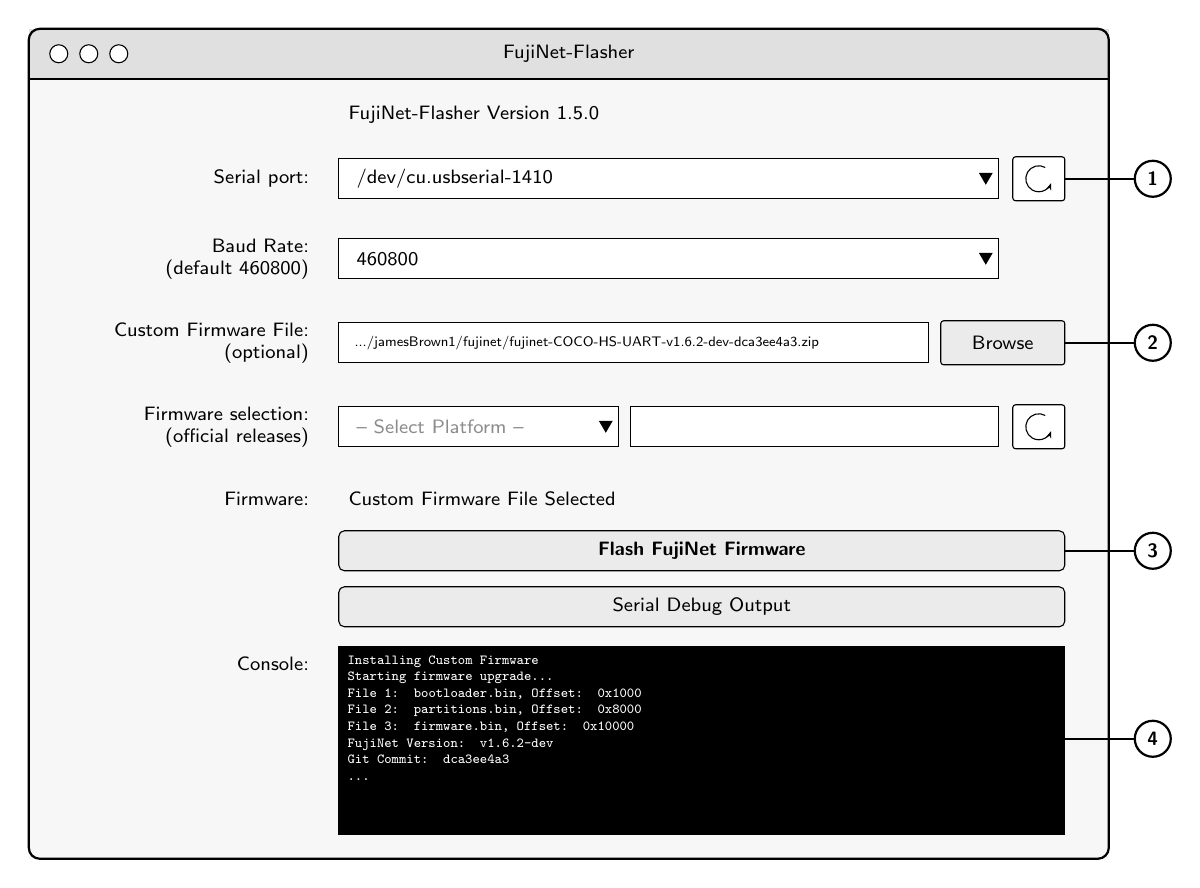
\begin{tikzpicture}[x=1in, y=1in, font=\sffamily\scriptsize]
  % the window
  \fill[black!3] (0,0) rectangle (5.4,3.9);
  \fill[black!12] (0,3.9) rectangle (5.4,4.15);
  \draw[thick] (0,3.9) -- (5.4,3.9);
  \draw[thick, rounded corners=4pt] (0,0) rectangle (5.4,4.15);
  \foreach \x in {0.15,0.3,0.45} \draw[fill=white] (\x,4.025) circle (0.045);
  \node at (2.7,4.025) {FujiNet-Flasher};
  \def\fx{1.55}
  \newcommand{\fwchoice}[3]{\draw[fill=white] (\fx,#1-0.1) rectangle (#2,#1+0.1);
    \node[anchor=west] at (\fx+0.04,#1) {#3};
    \fill ($(#2,#1)+(-0.1,0.03)$) -- ++(0.07,0) -- ++(-0.035,-0.06) -- cycle;}
  \newcommand{\fwreload}[1]{\draw[fill=white, rounded corners=1pt] (4.92,#1-0.11) rectangle (5.18,#1+0.11);
    \draw[-{Stealth[length=2.5pt]}, thin] (5.05,#1)++(60:0.065) arc[start angle=60, end angle=340, radius=0.065];}
  \node[anchor=west] at (\fx,3.72) {FujiNet-Flasher Version 1.5.0};
  \node[anchor=east] at (1.45,3.4) {Serial port:};
  \fwchoice{3.4}{4.85}{/dev/cu.usbserial-1410}\fwreload{3.4}
  \node[anchor=east, align=right] at (1.45,3.0) {Baud Rate:\\(default 460800)};
  \fwchoice{3.0}{4.85}{460800}
  \node[anchor=east, align=right] at (1.45,2.58) {Custom Firmware File:\\(optional)};
  \draw[fill=white] (\fx,2.48) rectangle (4.5,2.68);
  \node[anchor=west, font=\sffamily\tiny] at (\fx+0.03,2.58)
    {.../jamesBrown1/fujinet/fujinet-COCO-HS-UART-v1.6.2-dev-dca3ee4a3.zip};
  \draw[fill=black!8, rounded corners=1pt] (4.56,2.47) rectangle (5.18,2.69)
    node[midway]{Browse};
  \node[anchor=east, align=right] at (1.45,2.16) {Firmware selection:\\(official releases)};
  \fwchoice{2.16}{2.95}{\textcolor{black!45}{-- Select Platform --}}
  \draw[fill=white] (3.01,2.06) rectangle (4.85,2.26);
  \fwreload{2.16}
  \node[anchor=east] at (1.45,1.8) {Firmware:};
  \node[anchor=west] at (\fx,1.8) {Custom Firmware File Selected};
  \draw[fill=black!8, rounded corners=2pt] (\fx,1.44) rectangle (5.18,1.64)
    node[midway, font=\sffamily\bfseries\scriptsize]{Flash FujiNet Firmware};
  \draw[fill=black!8, rounded corners=2pt] (\fx,1.16) rectangle (5.18,1.36)
    node[midway]{Serial Debug Output};
  \node[anchor=north east] at (1.45,1.06) {Console:};
  \draw[fill=black] (\fx,0.12) rectangle (5.18,1.06);
  \node[anchor=north west, text=white, align=left, font=\ttfamily\tiny,
    inner sep=3pt] at (\fx,1.06)
    {Installing Custom Firmware\\Starting firmware upgrade...\\
     File 1: bootloader.bin, Offset: 0x1000\\File 2: partitions.bin, Offset: 0x8000\\
     File 3: firmware.bin, Offset: 0x10000\\FujiNet Version: v1.6.2-dev\\
     Git Commit: dca3ee4a3\\...};
  % callouts
  \foreach \n/\y in {1/3.4, 2/2.58, 3/1.54, 4/0.6} {
    \draw[thick] (5.18,\y) -- (5.55,\y);
    \node[callout] at (5.62,\y) {\n};
  }
\end{tikzpicture}
\caption{FujiNet-Flasher, ready to flash: (1) the DevKitC's serial port; (2)
the firmware from the release; (3) the button that flashes it; (4) its
progress, and then the FujiNet's log}\label{fig:flasher}
\end{figure}

FujiNet-Flasher erases the whole of the ESP32's flash, writes the five
parts of the firmware---\file{bootloader.bin}, \file{partitions.bin},
\file{firmware.bin}, \file{update.bin}, and \file{littlefs.bin}, the web
pages---restarts the ESP32, and shows its log in the console. It takes a
few minutes. At the end the console says:
\begin{exsmall}
Hard Resetting...
Done! Flashing is complete!
\end{exsmall}

\note{Erasing the flash also erases the settings the FujiNet keeps there.
The copy of its settings on its SD card, \file{fnconfig.ini}, is not
touched, and the FujiNet reads it again when it starts.}

If FujiNet-Flasher cannot find the ESP32 (\texttt{Error Detecting ESP}),
hold down the DevKitC's \key{BOOT} button, press and let go of \key{EN},
let go of \key{BOOT}, and click \key{Flash FujiNet Firmware} again. A
lower baud rate, such as 115200, sometimes helps with a long cable.

\section{Checking the Firmware}

The console shows the FujiNet's log as it starts; \key{Serial Debug
Output} shows it again whenever you click it (and restarts the ESP32). It
should include these lines:
\begin{exsmall}
FujiNet v1.6.2-dev 2026-06-18 09:35:40 (COCO) Started @ 9
LittleFS mounted.
[lib/bus/drivewire/drivewire.cpp:827] readBaudSwitch(): COCO_HS_UART build, defaulting to 921600 baud
\end{exsmall}
The first says which firmware it is; the last, that it is the build for
the TFR/911H. Without an SD card it also says that it found none; you
make the card in the next chapter.

Close FujiNet-Flasher before you go on: only one program at a time can
have the serial port open, and opening it restarts the ESP32.

% ═══════════════════════════════════════════════════════════════════
\chapter{Making the SD Card}
\chapterpages
\renewcommand{\thesectname}{Making the SD Card}

The FujiNet's SD card holds the disk that NitrOS-9 boots from and the
FujiNet's settings. This chapter describes how to make it on your
computer, with a card reader. Section~\ref{sec:webdav} tells how to do
the same over WiFi instead.

\section{Formatting the Card}

Use a microSD card of 32~GB or less, formatted FAT32. A new card usually
is. To format one:

\begin{keys}[1.1in]
macOS & In Disk Utility, choose \key{View}, then \key{Show All Devices};
choose the card (the device, not a volume on it), click \key{Erase}, and
choose the format \sans{MS-DOS (FAT)} and the scheme \sans{Master Boot
Record}. Name it \texttt{FUJINET}.\\
Linux & Find the card's device with \type{lsblk}, then, if it is
\file{/dev/sdb} with one partition: \type{sudo mkfs.vfat -F 32 -n FUJINET
/dev/sdb1}. Check the device name twice; this erases it.\\
\end{keys}

\section{Copying the Files}

Copy everything in the release's \file{sdcard/} folder to the top of the
card, keeping the folder \file{tfr911}. Figure~\ref{fig:card} shows the
card when you are done.

\begin{ex}
$ \textbf{cd jamesBrown1}
$ \textbf{cp -R sdcard/ /Volumes/FUJINET/}               \textrm{\small (macOS)}
$ \textbf{cp -R sdcard/. /media/\$USER/FUJINET/}         \textrm{\small (Linux)}
\end{ex}

\begin{figure}[htbp]
\centering
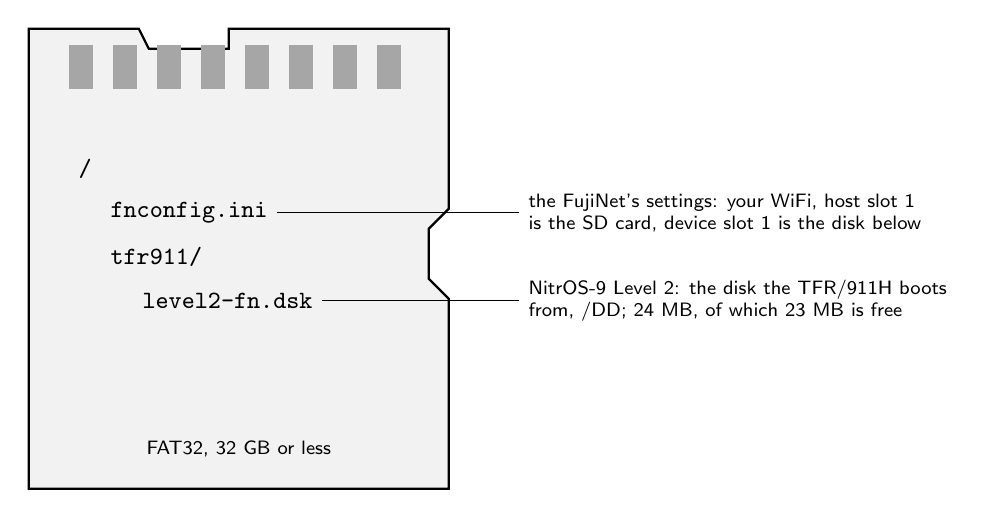
\begin{tikzpicture}[x=1in, y=1in, font=\sffamily\small]
  % a microSD card, its notched outline, big
  \draw[thick, fill=black!5] (0,0) -- (0,2.3) -- (0.55,2.3) -- (0.6,2.2)
    -- (1.0,2.2) -- (1.0,2.3) -- (2.1,2.3) -- (2.1,1.4) -- (2.0,1.3)
    -- (2.0,1.05) -- (2.1,0.95) -- (2.1,0) -- cycle;
  \foreach \x in {0.2,0.42,...,1.95} \fill[black!35] (\x,2.0) rectangle ++(0.12,0.22);
  \node[anchor=west, font=\ttfamily\small] at (0.2,1.6) {/};
  \node[anchor=west, font=\ttfamily\small] (ini) at (0.36,1.38) {fnconfig.ini};
  \node[anchor=west, font=\ttfamily\small] at (0.36,1.16) {tfr911/};
  \node[anchor=west, font=\ttfamily\small] (dsk) at (0.52,0.94) {level2-fn.dsk};
  \node[font=\sffamily\scriptsize] at (1.05,0.2) {FAT32, 32 GB or less};
  % what each is
  \draw[thin] (ini.east) -- (2.45,1.38) node[right, align=left, font=\sffamily\scriptsize]
    {the FujiNet's settings: your WiFi, host slot 1\\is the SD card, device slot 1 is the disk below};
  \draw[thin] (dsk.east) -- (2.45,0.94) node[right, align=left, font=\sffamily\scriptsize]
    {NitrOS-9 Level 2: the disk the TFR/911H boots\\from, /DD; 24 MB, of which 23 MB is free};
\end{tikzpicture}
\caption{The FujiNet's SD card}\label{fig:card}
\end{figure}

The disk image is about 500~KB as a file, but it is a 24~MB disk to
NitrOS-9: the file grows as NitrOS-9 fills it.

\section{The FujiNet's Settings}

\file{fnconfig.ini} holds the FujiNet's settings. The one in the release
sets three things: your WiFi network, host slot~1 (the SD card), and
device slot~1 (the boot disk). Open it in a text editor (TextEdit on a
Mac, in plain text) and put your network's name and password in place of
\texttt{YOUR-NETWORK} and \texttt{YOUR-PASSWORD}:

\begin{ex}
[WiFi]
enabled=1
SSID=\textbf{\var{your network's name}}
passphrase=\textbf{\var{its password}}
\end{ex}

The rest of the file is set already:

\begin{keys}[1.35in]
\texttt{[General]} & The FujiNet's name on your network,
\texttt{fujinet-tfr911}; \texttt{encrypt\_passphrase=0}, so that the
password above is read as you typed it.\\
\texttt{[Host1]} & Host slot~1 is the SD card. \texttt{[Host2]} is the
FujiNet project's TNFS server, \texttt{fujinet.online}.\\
\texttt{[Mount1]} & Device slot~1 holds \file{/tfr911/level2-fn.dsk}, from
host slot~1, read and write (\texttt{mode=w}). Device slot~1 is
DriveWire drive~0, \file{/X0} to NitrOS-9, and it is the slot the
TFR/911H boots from.\\
\end{keys}

Appendix~C lists every setting the file uses. The FujiNet reads the file
from the SD card each time it starts, copies it to its flash, and writes
both copies again when its settings change, without the notes at the top.

\note{The password is stored on the card as plain text. Anyone with the
card can read it.}

To boot without WiFi, change \texttt{enabled=1} in the \texttt{[WiFi]}
section to \texttt{enabled=0}. NitrOS-9 boots and runs as well, but the
network programs have nothing to talk to. You can set the WiFi later from
NitrOS-9 (Section~\ref{sec:wifi}).

\section{Putting the Card in the FujiNet}

Eject the card from your computer, put it in the FujiNet's slot, and
press the DevKitC's \key{EN} button (or unplug its USB and plug it in
again). If you watch its log (\key{Serial Debug Output} in FujiNet-Flasher),
it says:
\begin{exsmall}
SD mounted.
Load fnconfig.ini from SD
...
WiFi connect attempt to SSID "\var{your network's name}"
...
Obtained IP address: \var{192.168.1.232}
Starting web server on port 80
\end{exsmall}
Write down the IP address. With it you can open the FujiNet's web page
(\file{http://}\var{address}\file{/}) and reach its SD card over WiFi.

\section{Doing It over WiFi}\label{sec:webdav}

Once the FujiNet is on your network, its web server offers its SD card by
WebDAV at \file{/dav}. To copy the boot disk to it from your computer, with
\var{address} the FujiNet's IP address:
\begin{ex}
$ \textbf{curl -X MKCOL http://\var{address}/dav/tfr911}
$ \textbf{curl -T sdcard/tfr911/level2-fn.dsk http://\var{address}/dav/tfr911/level2-fn.dsk}
\end{ex}
Then put the disk in device slot~1, read and write, on the FujiNet's web
page, or from NitrOS-9 booted from the tether's disk (Section~\ref{sec:l2}):
\begin{ex}
OS9: \textbf{fnsetdevfile 0 1 2 /tfr911/level2-fn.dsk}
\end{ex}
(\cmd{fnsetdevfile} counts device slots from~0: slot~0 is the FujiNet's
slot~1. Host slot~1 is the SD card, and mode~2 is read/write.)

The same way, \type{curl -o level2-fn-backup.dsk
http://\var{address}/dav/tfr911/level2-fn.dsk} copies the disk back to
your computer, to keep a backup.

% ═══════════════════════════════════════════════════════════════════
\chapter{Preparing the TFR/911H}
\chapterpages
\renewcommand{\thesectname}{Preparing the TFR/911H}

This chapter describes how to flash the TFR/911H's firmware and install
the tether, and how to check that they work before the FujiNet is
connected.

\section{The Board}

Figure~\ref{fig:board} shows the parts of the TFR/911H this guide uses:
the USB-C connector, through which the board takes its power and talks
to the tether; the \key{RESET} and \key{FLASH} buttons; and header J3,
the 20-pin socket at the lower left, where the FujiNet connects.

\begin{figure}[htbp]
\centering
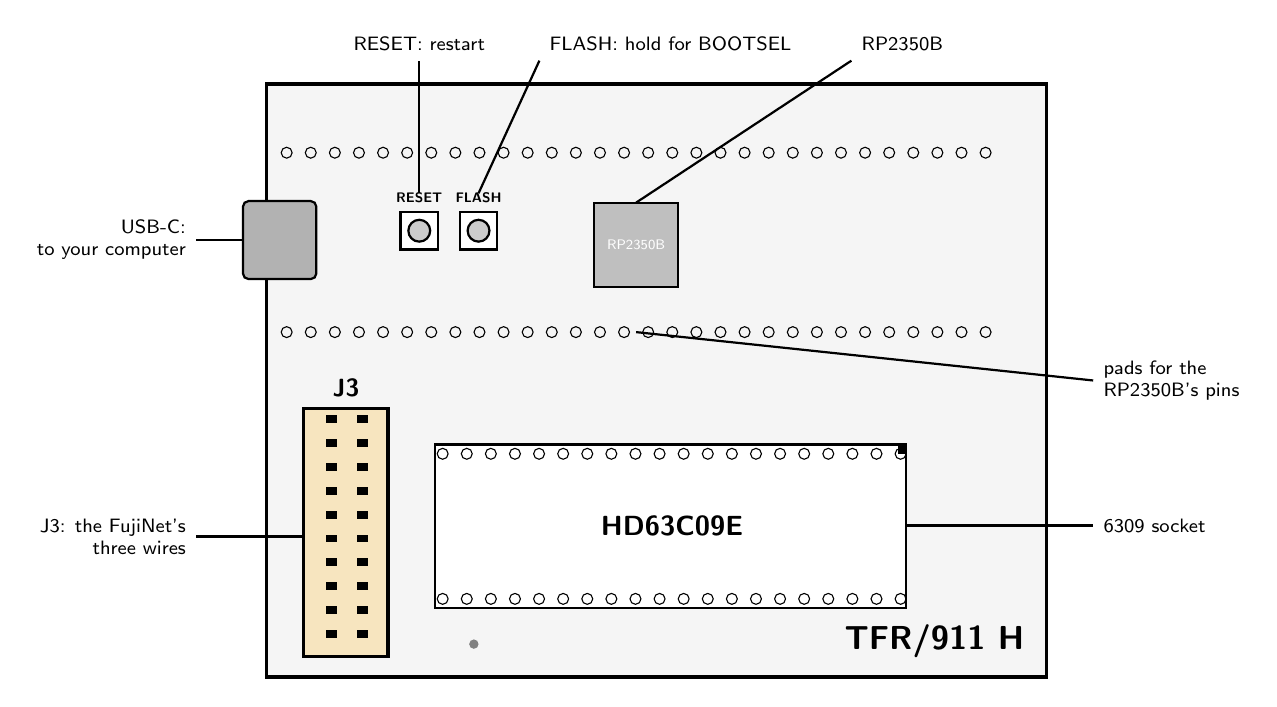
\begin{tikzpicture}[x=0.78in, y=0.78in, font=\sffamily\scriptsize]
  % the board, from its layout, 5 by 3.8
  \draw[very thick, fill=black!4] (0,0) rectangle (5.0,3.8);
  % USB-C at the left
  \draw[thick, fill=black!30, rounded corners=2pt] (-0.15,2.55) rectangle (0.32,3.05);
  % the buttons, RESET and FLASH
  \foreach \x/\l in {0.98/RESET, 1.36/FLASH} {
    \draw[thick, fill=white] (\x-0.12,2.74) rectangle (\x+0.12,2.98);
    \draw[thick, fill=black!20] (\x,2.86) circle (0.07);
    \node[font=\sffamily\bfseries\tiny, above] at (\x,2.98) {\l};
  }
  % the RP2350B and its rows of pads
  \draw[thick, fill=black!25] (2.1,2.5) rectangle (2.64,3.04);
  \node[font=\sffamily\tiny, text=white] at (2.37,2.77) {RP2350B};
  \foreach \i in {0,...,29} {
    \draw (0.13+\i*0.1545,3.36) circle (0.035);
    \draw (0.13+\i*0.1545,2.21) circle (0.035);
  }
  % the 63C09E in its socket
  \draw[thick, fill=white] (1.08,0.44) rectangle (4.1,1.49);
  \foreach \i in {0,...,19} {
    \draw (1.13+\i*0.1545,1.43) circle (0.035);
    \draw (1.13+\i*0.1545,0.50) circle (0.035);
  }
  \node[font=\sffamily\bfseries] at (2.6,0.97) {HD63C09E};
  \fill (4.05,1.43) rectangle ++(0.05,0.05);
  % J3, 2 by 10, at the lower left
  \draw[very thick, fill=wiretx!25] (0.24,0.13) rectangle (0.78,1.72);
  \foreach \r in {0,...,9} {
    \fill (0.38,0.25+\r*0.153) rectangle ++(0.07,0.05);
    \fill (0.58,0.25+\r*0.153) rectangle ++(0.07,0.05);
  }
  \node[font=\sffamily\bfseries\small] at (0.51,1.85) {J3};
  % LED, and the name
  \fill[black!50] (1.33,0.21) circle (0.03);
  \node[font=\sffamily\bfseries\large, anchor=south east] at (4.92,0.06) {TFR/911 H};
  % callouts
  \draw[thick] (-0.15,2.8) -- (-0.45,2.8) node[left, align=right]{USB-C:\\to your computer};
  \draw[thick] (0.98,3.1) -- (0.98,3.95) node[above]{RESET: restart};
  \draw[thick] (1.36,3.1) -- (1.75,3.95) node[above right, align=left]{FLASH: hold for BOOTSEL};
  \draw[thick] (0.24,0.9) -- (-0.45,0.9) node[left, align=right]{J3: the FujiNet's\\three wires};
  \draw[thick] (2.37,3.04) -- (3.75,3.95) node[above right]{RP2350B};
  \draw[thick] (4.1,0.97) -- (5.3,0.97) node[right, align=left]{6309 socket};
  \draw[thick] (2.37,2.21) -- (5.3,1.9) node[right, align=left]{pads for the\\RP2350B's pins};
\end{tikzpicture}
\caption{The TFR/911H, seen from above}\label{fig:board}
\end{figure}

\section{Flashing the Firmware}

The TFR/911H's firmware is \file{tfr911h/tfr911h\_v4.uf2}. It holds the
firmware's console (the \texttt{TCL>} prompt), its two NitrOS-9 kernels,
one booting from the tether's disk (\cmd{l2}) and one from the FujiNet
(\cmd{l2fn}), and the becker port through which the 6309 talks to the
FujiNet.

The RP2350B has a boot loader in ROM, BOOTSEL, which makes the board look
like a USB drive. Copying a \file{.uf2} file to that drive flashes the
firmware. Figure~\ref{fig:bootsel} shows how to start BOOTSEL with the
board's two buttons.

\begin{figure}[htbp]
\centering
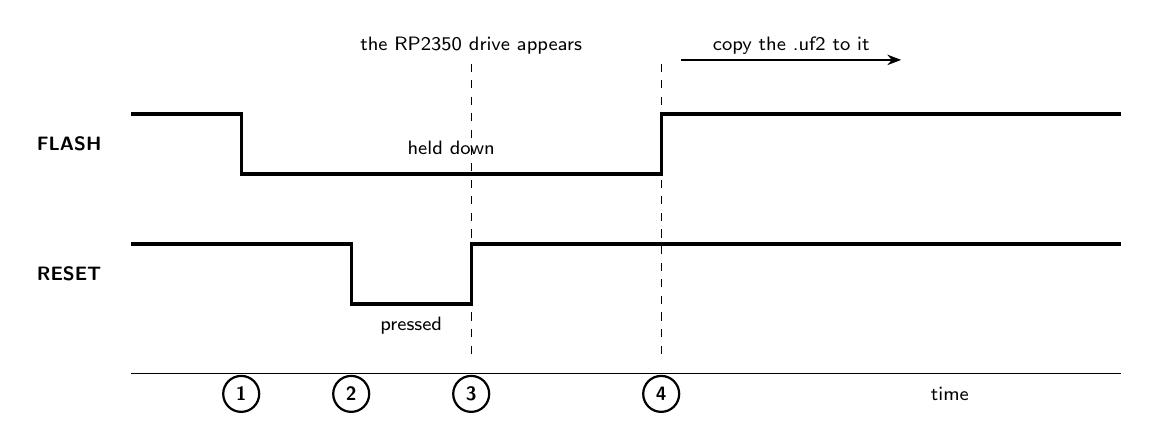
\begin{tikzpicture}[x=1in, y=1in, font=\sffamily\scriptsize]
  % time runs to the right; a button low is a button held down
  \node[anchor=east, font=\sffamily\bfseries\scriptsize] at (0.55,1.2) {FLASH};
  \node[anchor=east, font=\sffamily\bfseries\scriptsize] at (0.55,0.55) {RESET};
  \draw[very thick] (0.65,1.35) -- (1.2,1.35) -- (1.2,1.05) -- (3.3,1.05)
    -- (3.3,1.35) -- (5.6,1.35);
  \draw[very thick] (0.65,0.7) -- (1.75,0.7) -- (1.75,0.4) -- (2.35,0.4)
    -- (2.35,0.7) -- (5.6,0.7);
  \node[lab] at (2.25,1.18) {held down};
  \node[lab] at (2.05,0.29) {pressed};
  \draw[dashed, thin] (2.35,0.15) -- (2.35,1.6);
  \draw[dashed, thin] (3.3,0.15) -- (3.3,1.6);
  \node[lab, anchor=south] at (2.35,1.6) {the RP2350 drive appears};
  \node[lab, anchor=south] at (3.95,1.6) {copy the .uf2 to it};
  \draw[arr] (3.4,1.62) -- (4.5,1.62);
  \foreach \x/\n in {1.2/1, 1.75/2, 2.35/3, 3.3/4} \node[callout] at (\x,-0.05) {\n};
  \draw[thin] (0.65,0.05) -- (5.6,0.05);
  \node[lab, anchor=west] at (4.6,-0.05) {time};
\end{tikzpicture}
\caption{Starting BOOTSEL: (1) hold down FLASH; (2) press RESET; (3) let
go of RESET; (4) let go of FLASH}\label{fig:bootsel}
\end{figure}

\begin{steps}
\item Plug the TFR/911H into your computer with the USB-C cable.
\item Hold down \key{FLASH}. Press and let go of \key{RESET}. Then let go
of \key{FLASH}. (Or hold down \key{FLASH} while you plug the cable in.)
\item A drive named \file{RP2350} appears on your computer.
\item Copy \file{tfr911h\_v4.uf2} to it, by dragging it in the Finder or
the file manager, or:
\begin{ex}
$ \textbf{cp tfr911h/tfr911h_v4.uf2 /Volumes/RP2350/}           \textrm{\small (macOS)}
$ \textbf{cp tfr911h/tfr911h_v4.uf2 /media/\$USER/RP2350/}       \textrm{\small (Linux)}
\end{ex}
\item The drive goes away by itself and the board restarts with the new
firmware. macOS may complain that the disk was not ejected properly;
that is expected, and does no harm.
\end{steps}

With Raspberry Pi's \cmd{picotool}, \type{picotool load -x
tfr911h/tfr911h\_v4.uf2} does steps 4 and 5, once the board is in
BOOTSEL.

\caution{Quit the tether before you flash the firmware: only one program
at a time can have the board's serial port open.}

\section{Installing the Tether}

The tether is a program on your computer that talks to the TFR/911H over
USB. It is the board's terminal: what you type goes to the 6309, and what
the 6309 prints appears in the tether's window. It also serves a disk
image on your computer to NitrOS-9 as \file{/H0}, and sets the board's
clock when it connects.

Copy the release's \file{tether/} folder anywhere you like; it holds
the tether for each kind of computer (Table~\ref{tab:tethers}), the disk
it serves, and \file{run-tfr.sh}, which starts it.

\begin{table}[H]
\caption{The tethers}\label{tab:tethers}
\begin{tabularx}{\linewidth}{@{}l X@{}}
\toprule
\textbf{File} & \textbf{For}\\
\midrule
\file{tether-darwin-arm64} & A Mac with Apple silicon (M1 and later)\\
\file{tether-darwin-amd64} & A Mac with an Intel processor\\
\file{tether-linux-amd64} & A Linux PC (x86-64)\\
\file{tether-linux-arm64} & 64-bit Linux on ARM: a Raspberry Pi 3, 4,
or 5 with a 64-bit system\\
\file{tether-linux-arm} & 32-bit Linux on ARMv7: a Raspberry Pi 2, 3, or
4 with a 32-bit system\\
\bottomrule
\end{tabularx}
\end{table}

\file{run-tfr.sh} chooses the right one. Before you run it the first
time:

\begin{keys}[1.1in]
macOS & Files downloaded from the Internet are quarantined, and macOS
will not run a quarantined program that is not signed. Take the release
out of quarantine:
\texttt{\textbf{xattr -dr com.apple.quarantine jamesBrown1}}\\
Linux & Your user must be in the group that owns the board's serial
port, \file{/dev/ttyACM0}: \type{sudo usermod -aG dialout \$USER}, then
log out and in again (on Arch Linux, the group \texttt{uucp}).\\
\end{keys}

The tether runs in a terminal window: Terminal or iTerm2 on a Mac, any
terminal on Linux. Make the window at least 80 columns by 24 lines; the
NitrOS-9 programs in the release draw full-screen, in color, with the
box-drawing characters of UTF-8, which the usual terminal fonts (Menlo,
SF Mono, DejaVu Sans Mono) all have.

\section{First Contact}

To check the firmware and the tether, run \file{run-tfr.sh} with
\texttt{none}, which connects without booting anything:
\begin{ex}
$ \textbf{cd jamesBrown1/tether}
$ \textbf{sh run-tfr.sh none}
TFR/911H on /dev/cu.usbmodem13401; disk .../level2.dsk; boot nothing.
^C goes to OS-9.  Quit with ^] .

TCL> \textbf{fujinet}
no answer from the FujiNet (0 of 6 bytes; GPIO 12 TX, 13 RX, 921600 baud)
TCL>
\end{ex}
If \texttt{TCL>} does not appear at once, press \key{Return}. The
\cmd{fujinet} command asks the FujiNet the time; with no FujiNet connected
yet, it has no answer. Quit the tether with \key{Ctrl/]}.

\file{run-tfr.sh} finds the board's serial device by itself when there is
only one: \file{/dev/cu.usbmodem*} on a Mac, \file{/dev/ttyACM*} on
Linux. If there are several, it lists them; set \texttt{WIRE} to the
right one:
\begin{ex}
$ \textbf{WIRE=/dev/cu.usbmodem13401 sh run-tfr.sh none}
\end{ex}

% ═══════════════════════════════════════════════════════════════════
\chapter{Connecting the FujiNet}
\chapterpages
\renewcommand{\thesectname}{Connecting the FujiNet}

This chapter describes how to wire the FujiNet to the TFR/911H with three
wires, how to power the two boards, and how to check the link between
them.

\section{Header J3}

The FujiNet connects to header J3, the 2-by-10 socket at the lower left
of the TFR/911H, beside the 6309 (Figure~\ref{fig:board}). The name of
each pin is printed beside it; Figure~\ref{fig:j3} shows them. Pin~1,
marked \pin{G8}, is at the bottom left; the odd pins run up the left
column and the even pins up the right.

\begin{figure}[htbp]
\centering
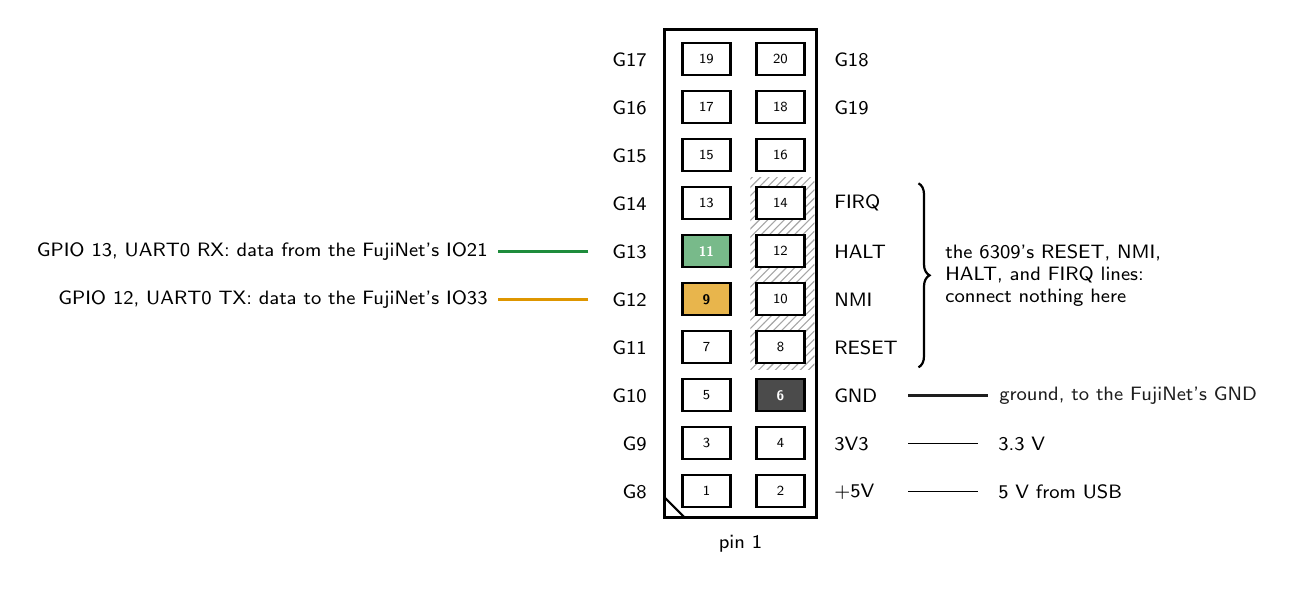
\begin{tikzpicture}[x=1in, y=1in, font=\sffamily\scriptsize]
  \def\p{0.24}
  % the 6309 signals: leave alone
  \fill[pattern=north east lines, pattern color=black!35] (0.41,3*\p) rectangle (0.73,7*\p);
  \draw[very thick, fill=none] (-0.02,-0.02) rectangle (0.74,10*\p+0.02);
  \draw[thick] (-0.02,0.08) -- (0.08,-0.02);  % the corner cut at pin 1
  \foreach \r [count=\i from 0] in {1,...,10} {
    \pgfmathtruncatemacro\odd{2*\i+1}
    \pgfmathtruncatemacro\even{2*\i+2}
    \draw[thick, fill=white] (0.07,\i*\p+0.03) rectangle ++(0.24,0.16)
      node[midway, font=\sffamily\tiny]{\odd};
    \draw[thick, fill=white] (0.44,\i*\p+0.03) rectangle ++(0.24,0.16)
      node[midway, font=\sffamily\tiny]{\even};
  }
  % the three we use
  \draw[thick, fill=wiretx!70] (0.07,4*\p+0.03) rectangle ++(0.24,0.16) node[midway, font=\sffamily\bfseries\tiny]{9};
  \draw[thick, fill=wirerx!60] (0.07,5*\p+0.03) rectangle ++(0.24,0.16) node[midway, font=\sffamily\bfseries\tiny, text=white]{11};
  \draw[thick, fill=wiregnd!80] (0.44,2*\p+0.03) rectangle ++(0.24,0.16) node[midway, font=\sffamily\bfseries\tiny, text=white]{6};
  % silkscreen names
  \foreach \l [count=\i from 0] in {G8,G9,G10,G11,G12,G13,G14,G15,G16,G17}
    \node[anchor=east] at (-0.06,\i*\p+0.11) {\l};
  \foreach \l [count=\i from 0] in {+5V,3V3,GND,RESET,NMI,HALT,FIRQ,{},G19,G18}
    \node[anchor=west] at (0.78,\i*\p+0.11) {\l};
  % what they are
  \draw[wiretx, very thick] (-0.4,4*\p+0.11) -- (-0.85,4*\p+0.11)
    node[left, text=black]{GPIO 12, UART0 TX: data to the FujiNet's IO33};
  \draw[wirerx, very thick] (-0.4,5*\p+0.11) -- (-0.85,5*\p+0.11)
    node[left, text=black]{GPIO 13, UART0 RX: data from the FujiNet's IO21};
  \draw[wiregnd, very thick] (1.2,2*\p+0.11) -- (1.6,2*\p+0.11)
    node[right, align=left]{ground, to the FujiNet's GND};
  \draw[decorate, decoration={brace, amplitude=4pt}, thick] (1.25,6*\p+0.21) -- (1.25,3*\p+0.01)
    node[midway, right=6pt, align=left]{the 6309's RESET, NMI,\\HALT, and FIRQ lines:\\connect nothing here};
  \node[align=left, anchor=west] at (1.6,0.11) {5 V from USB};
  \draw[thin] (1.2,0.11) -- (1.55,0.11);
  \node[align=left, anchor=west] at (1.6,1*\p+0.11) {3.3 V};
  \draw[thin] (1.2,1*\p+0.11) -- (1.55,1*\p+0.11);
  \node[anchor=north] at (0.36,-0.06) {pin 1};
\end{tikzpicture}
\caption{Header J3, seen from above, with the 6309 to the right}\label{fig:j3}
\end{figure}

Three of J3's pins carry the link to the FujiNet: \pin{G12} (pin~9),
\pin{G13} (pin~11), and \pin{GND} (pin~6).

\caution{Pins 8, 10, 12, and 14 are wired to the 6309's RESET, NMI,
HALT, and FIRQ lines. Connect nothing to them. Do not connect the 3V3 or
+5V pins to the FujiNet either: each board takes its power from its own
USB cable.}

\section{Wiring}

Figure~\ref{fig:wiring} and Table~\ref{tab:wires} show the three wires.
Each data wire goes from one board's transmit pin to the other's receive
pin; the table has that crossing in it already, so wire it just as it
says.

\begin{figure}[htbp]
\centering
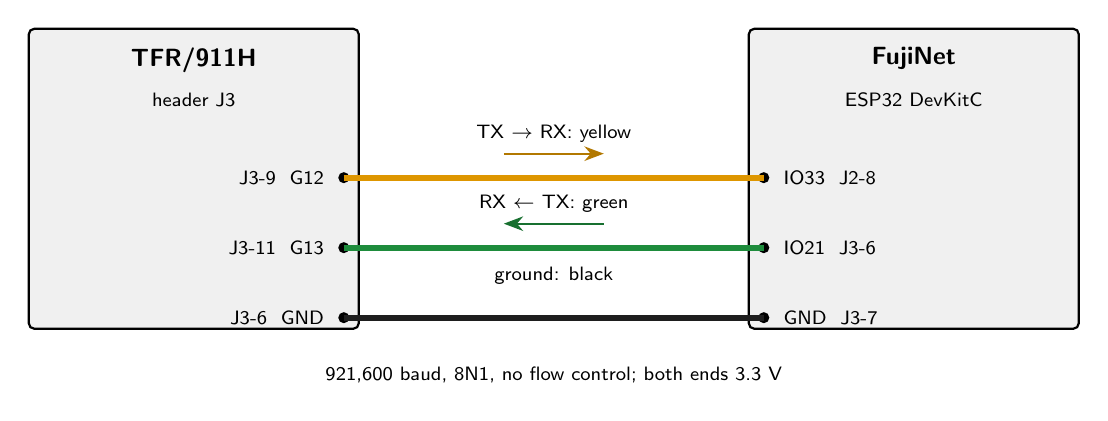
\begin{tikzpicture}[x=1in, y=1in, font=\sffamily\scriptsize]
  \node[box, minimum width=1.65in, minimum height=1.5in, anchor=north] (t) at (0.8,1.6) {};
  \node[font=\sffamily\bfseries\small, anchor=north] at (0.8,1.55) {TFR/911H};
  \node[anchor=north] at (0.8,1.32) {header J3};
  \node[box, minimum width=1.65in, minimum height=1.5in, anchor=north] (f) at (4.4,1.6) {};
  \node[font=\sffamily\bfseries\small, anchor=north] at (4.4,1.55) {FujiNet};
  \node[anchor=north] at (4.4,1.32) {ESP32 DevKitC};
  \foreach \y/\a/\b/\c/\d in {0.85/{J3-9\ \ G12}/{IO33\ \ J2-8}/wiretx/1,
                              0.5/{J3-11\ \ G13}/{IO21\ \ J3-6}/wirerx/-1,
                              0.15/{J3-6\ \ GND}/{GND\ \ J3-7}/wiregnd/0} {
    \fill (1.55,\y) circle (2pt);
    \fill (3.65,\y) circle (2pt);
    \node[anchor=east] at (1.5,\y) {\a};
    \node[anchor=west] at (3.7,\y) {\b};
    \draw[\c, line width=2.2pt] (1.55,\y) -- (3.65,\y);
  }
  \draw[-{Stealth[length=7pt]}, wiretx!80!black, thick] (2.35,0.97) -- (2.85,0.97);
  \node[lab, anchor=south] at (2.6,0.98) {TX $\rightarrow$ RX: yellow};
  \draw[-{Stealth[length=7pt]}, wirerx!80!black, thick] (2.85,0.62) -- (2.35,0.62);
  \node[lab, anchor=south] at (2.6,0.63) {RX $\leftarrow$ TX: green};
  \node[lab, anchor=south] at (2.6,0.27) {ground: black};
  \node[lab, anchor=north, align=center] at (2.6,-0.05)
    {921{,}600 baud, 8N1, no flow control; both ends 3.3 V};
\end{tikzpicture}
\caption{The three wires between the TFR/911H and the FujiNet}\label{fig:wiring}
\end{figure}

\begin{table}[H]
\caption{The wires}\label{tab:wires}
\begin{tabularx}{\linewidth}{@{}l l l l X@{}}
\toprule
\textbf{TFR/911H} & \textbf{Signal} & \textbf{FujiNet} & \textbf{Signal} & \textbf{Wire}\\
\midrule
\pin{J3-9}, \pin{G12} & GPIO~12, UART0 TX & \pin{IO33}, \pin{J2-8} & GPIO~33, UART1 RX & yellow\\
\pin{J3-11}, \pin{G13} & GPIO~13, UART0 RX & \pin{IO21}, \pin{J3-6} & GPIO~21, UART1 TX & green\\
\pin{J3-6}, \pin{GND} & ground & \pin{GND}, \pin{J3-7} & ground & black\\
\bottomrule
\end{tabularx}
\end{table}

\begin{steps}
\item Unplug both boards from USB.
\item Push the female end of the yellow wire onto the DevKitC's
\pin{IO33}, the eighth pin down on the left, counting from the antenna
end (Figure~\ref{fig:devkitc}). Push its male end into J3 pin~9,
\pin{G12}.
\item Push the female end of the green wire onto the DevKitC's
\pin{IO21}, the sixth pin down on the right. Push its male end into J3
pin~11, \pin{G13}.
\item Push the female end of the black wire onto the DevKitC's
\pin{GND}, the seventh pin down on the right. Push its male end into J3
pin~6, \pin{GND}.
\item Check each wire against Table~\ref{tab:wires} before you plug
anything in.
\end{steps}

Any of the DevKitC's \pin{GND} pins will do for the ground wire. Keep the
wires short, 15~cm (6 inches) or less: the link runs at 921{,}600 baud.

\section{Power}

Each board takes its power from its own USB cable, and the ground wire
joins the two. Plug the FujiNet in first, so that it has started---a
few seconds---before the TFR/911H first asks it for something; then the
TFR/911H.

The FujiNet's USB cable can go to your computer, where it also carries
the FujiNet's log, or to any USB charger.

\caution{Keep the FujiNet powered while NitrOS-9 runs from it. NitrOS-9
waits for each answer from the FujiNet with nothing else running, and a
FujiNet that stops answering stops NitrOS-9 with it. If that happens,
press \key{RESET} on the TFR/911H and boot again.}

\section{Checking the Link}

Run \file{run-tfr.sh} with \texttt{none} again, and at the \texttt{TCL>}
prompt try the \cmd{fujinet} commands:
\begin{ex}
$ \textbf{sh run-tfr.sh none}
TCL> \textbf{fujinet}
FujiNet says it is 2026-10-20 19:41:07
TCL> \textbf{fujinet mount 1}
slot 1: mounted level2-fn.dsk
TCL> \textbf{fujinet stats}
rx \var{n} tx \var{n} rx_drops 0 tx_drops 0 overruns 0 empty_reads 0
\end{ex}

\begin{keys}[1.25in]
\cmd{fujinet} & Asks the FujiNet the time (DriveWire's \texttt{OP\_TIME})
and prints its answer. An answer proves both data wires, the ground, and
the baud rate. The time is the FujiNet's own, which it sets from the
network; without WiFi it starts in 1970, which does no harm.\\
\cmd{fujinet mount 1} & Mounts the disk in device slot~1, as booting
will. It proves the SD card, \file{fnconfig.ini}, and the disk.\\
\cmd{fujinet stats} & Counts the bytes each way, and any lost. The four
error counts should stay at~0.\\
\end{keys}

If \cmd{fujinet} has no answer, see Chapter~7.

% ═══════════════════════════════════════════════════════════════════
\chapter{Booting from the FujiNet}
\chapterpages
\renewcommand{\thesectname}{Booting from the FujiNet}

This chapter describes how to boot NitrOS-9 from the FujiNet, what
happens when you do, where everything is afterwards, and what to try
first.

\section{Booting}

With the FujiNet powered and connected, run \file{run-tfr.sh} with no
argument. It starts the tether and types \cmd{l2fn} at the
\texttt{TCL>} prompt for you:
\begin{ex}
$ \textbf{cd jamesBrown1/tether}
$ \textbf{sh run-tfr.sh}
TFR/911H on /dev/cu.usbmodem13401; disk .../level2.dsk; boot l2fn.
^C goes to OS-9.  Quit with ^] .
[Injecting: l2fn]
FujiNet slot 1: level2-fn.dsk
[L2: starting 6309 with NitrOS-9 Level 2]
[bye: asserting RESET+HALT...]
   ...
[bye: Phase 2 started]
L2FN
NitrOS-9/6809 Level 2 V03.3.0
Tandy Color Computer 3
(C) 2014 The NitrOS-9 Project
Tue Oct 20 19:42:16 2026
http://www.nitros9.org

NitrOS-9 Level 2 on the TFR/911H.  Unix-style commands: man unix
Shell

OS9:
\end{ex}

The lines in brackets are the firmware's, as it hands the board to the
6309; \texttt{L2FN} is the first thing the 6309 prints. NitrOS-9 is
running, from the FujiNet's SD card. (\texttt{Tandy Color
Computer~3} is the machine NitrOS-9 was built for; the TFR/911H's
firmware presents the 6309 with what NitrOS-9 needs of one.)

At \texttt{TCL>} you can also type \cmd{l2fn} yourself, after
\type{sh run-tfr.sh none}.

\section{What Happens}

Figure~\ref{fig:boot} shows what happens between \cmd{l2fn} and the
\texttt{OS9:} prompt.

\begin{figure}[htbp]
\centering
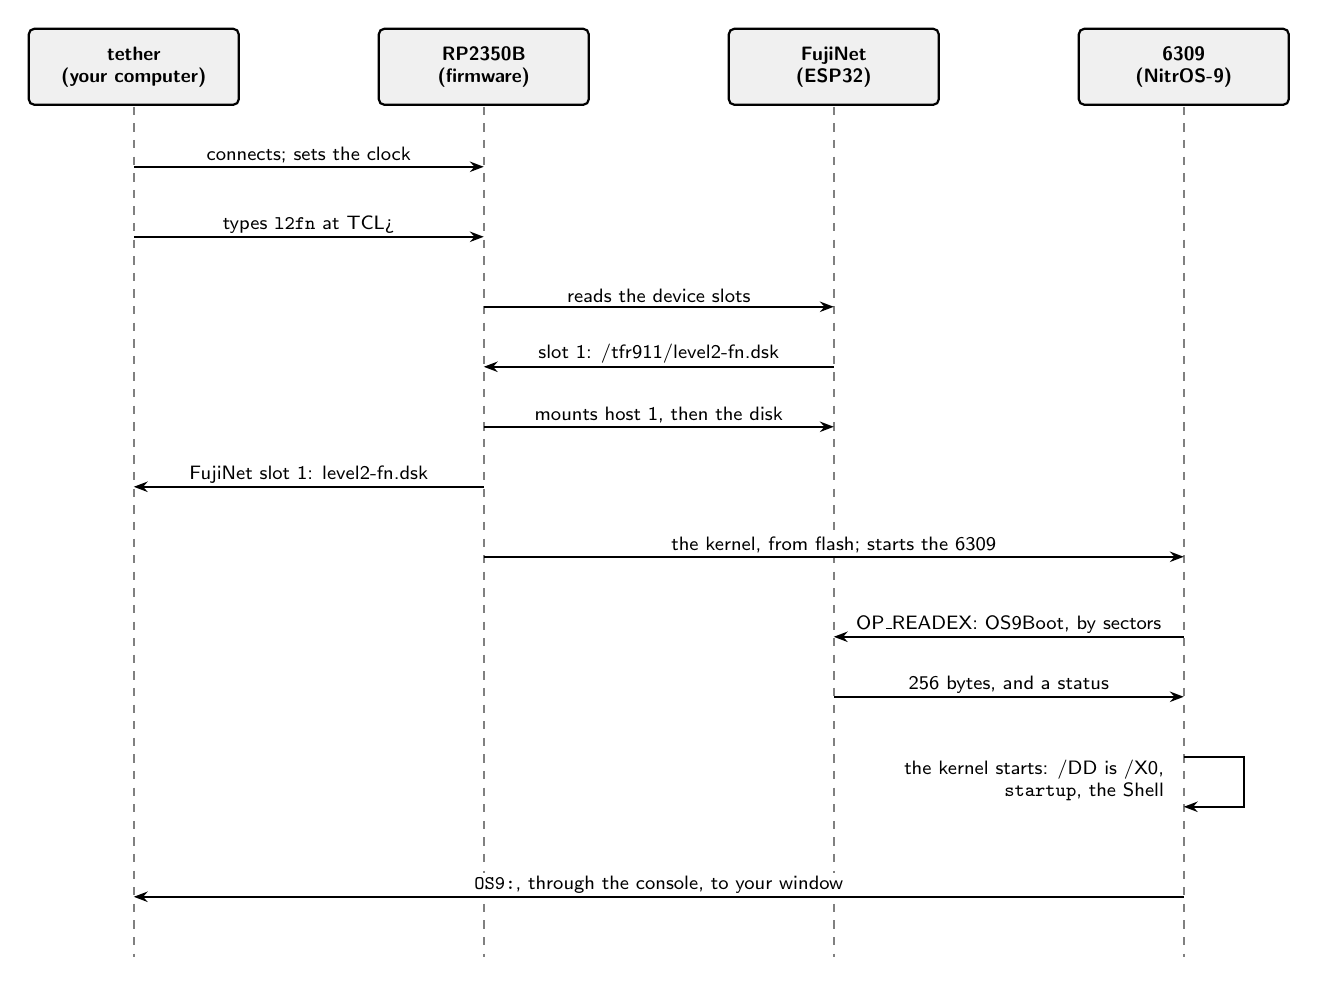
\begin{tikzpicture}[x=1in, y=1in, font=\sffamily\scriptsize]
  \foreach \x/\t in {0/{tether\\(your computer)}, 1.75/{RP2350B\\(firmware)},
                     3.5/{FujiNet\\(ESP32)}, 5.25/{6309\\(NitrOS-9)}} {
    \node[box, minimum width=1.05in, minimum height=0.38in, font=\sffamily\bfseries\scriptsize]
      at (\x,0) {\t};
    \draw[thick, dashed, black!50] (\x,-0.2) -- (\x,-4.45);
  }
  \newcommand{\bootmsg}[4]{\draw[arr] (#1,#3) -- (#2,#3)
    node[midway, above, lab, fill=white, inner sep=1pt]{#4};}
  \bootmsg{0}{1.75}{-0.5}{connects; sets the clock}
  \bootmsg{0}{1.75}{-0.85}{types \texttt{l2fn} at TCL>}
  \bootmsg{1.75}{3.5}{-1.2}{reads the device slots}
  \bootmsg{3.5}{1.75}{-1.5}{slot 1: /tfr911/level2-fn.dsk}
  \bootmsg{1.75}{3.5}{-1.8}{mounts host 1, then the disk}
  \bootmsg{1.75}{0}{-2.1}{FujiNet slot 1: level2-fn.dsk}
  \bootmsg{1.75}{5.25}{-2.45}{the kernel, from flash; starts the 6309}
  \bootmsg{5.25}{3.5}{-2.85}{OP\_READEX: OS9Boot, by sectors}
  \bootmsg{3.5}{5.25}{-3.15}{256 bytes, and a status}
  \draw[arr] (5.25,-3.45) -- ++(0.3,0) -- ++(0,-0.25) -- ++(-0.3,0);
  \node[lab, anchor=east, align=right] at (5.2,-3.57) {the kernel starts: /DD is /X0,\\\texttt{startup}, the Shell};
  \bootmsg{5.25}{0}{-4.15}{\texttt{OS9:}, through the console, to your window}
\end{tikzpicture}
\caption{Booting from the FujiNet}\label{fig:boot}
\end{figure}

\begin{steps}
\item The tether connects to the board and sets its clock. Given
\texttt{-boot l2fn}, it types \cmd{l2fn} at the \texttt{TCL>} prompt.
\item When the FujiNet starts, it puts its own CONFIG disk in DriveWire
drive~0. So \cmd{l2fn} first asks the FujiNet which disk device slot~1
names, mounts that slot's host (the SD card), then the disk, read and
write, and prints \texttt{FujiNet slot 1: level2-fn.dsk}.
\item The firmware copies NitrOS-9's kernel into the 6309's memory from
its own flash, and starts the 6309.
\item The kernel's \file{Boot} module, \file{boot\_dw}, reads the file
\file{OS9Boot} from DriveWire drive~0, a sector at a time, through the
becker port at \file{\$FF45}--\file{\$FF46} that the firmware makes of
the link.
\item \file{OS9Boot} names \file{/X0}, the FujiNet's slot~1, as
\file{/DD}, the system disk. NitrOS-9 runs \file{startup} from it, then
the Shell, whose \texttt{OS9:} prompt comes to your window through the
tether.
\end{steps}

\section{Where Everything Is}

Figure~\ref{fig:devices} shows what NitrOS-9's devices are, booted from
the FujiNet.

\begin{figure}[htbp]
\centering
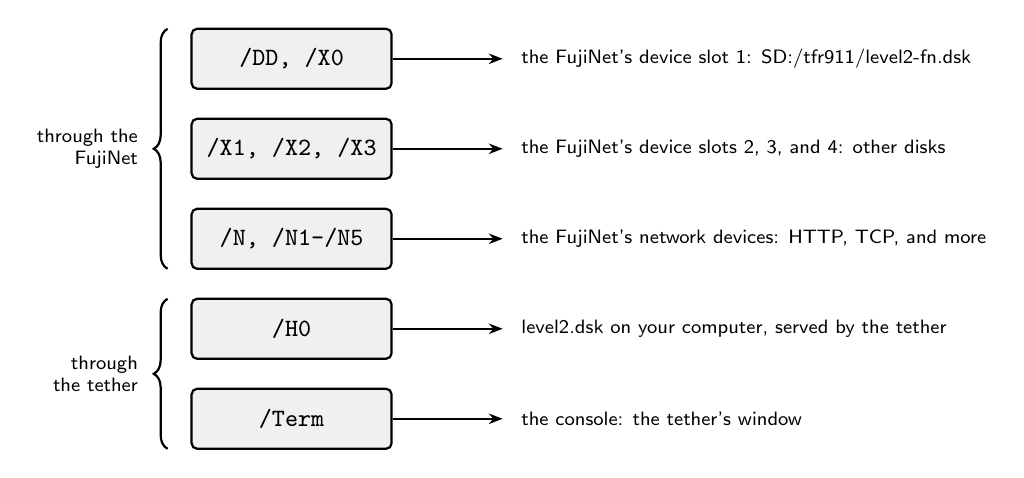
\begin{tikzpicture}[x=1in, y=1in, font=\sffamily\scriptsize]
  \foreach \y/\d/\w in {0/{/DD, /X0}/{the FujiNet's device slot 1: SD:/tfr911/level2-fn.dsk},
                        -0.45/{/X1, /X2, /X3}/{the FujiNet's device slots 2, 3, and 4: other disks},
                        -0.9/{/N, /N1-/N5}/{the FujiNet's network devices: HTTP, TCP, and more},
                        -1.35/{/H0}/{level2.dsk on your computer, served by the tether},
                        -1.8/{/Term}/{the console: the tether's window}} {
    \node[box, minimum width=1.0in, minimum height=0.3in, font=\ttfamily\small] (d) at (0,\y) {\d};
    \draw[arr] (d.east) -- ++(0.55,0);
    \node[anchor=west] at (1.1,\y) {\w};
  }
  \draw[decorate, decoration={brace, amplitude=5pt, mirror}, thick]
    (-0.62,0.15) -- (-0.62,-1.05) node[midway, left=7pt, align=right]{through the\\FujiNet};
  \draw[decorate, decoration={brace, amplitude=5pt, mirror}, thick]
    (-0.62,-1.2) -- (-0.62,-1.95) node[midway, left=7pt, align=right]{through\\the tether};
\end{tikzpicture}
\caption{NitrOS-9's devices, booted from the FujiNet}\label{fig:devices}
\end{figure}

Everything you save in \file{/DD} goes to \file{level2-fn.dsk} on the
FujiNet's SD card. \file{/H0} is a second disk with the same system on
it, on your computer: \type{dir /h0} shows it, and \type{copy /h0/}\var{file}
\type{/dd/}\var{file} copies from it.

\section{Trying It Out}

\begin{keys}[1.25in]
\cmd{fnstatus} & The FujiNet's firmware version, its WiFi network, and
its IP address.\\
\cmd{fnweather} & The weather where you are, now and for the week, with
pictures.\\
\cmd{fnnews} & The news.\\
\cmd{fnbattleship} & Fuji Battleship: sea battle for up to four players,
on the Internet, in color, with sound if your board has a speaker.\\
\cmd{fnbounce} & Bounce World: shapes bouncing from one computer's screen
to the next.\\
\cmd{fnstocks} & Ten stock quotes and a ticker.\\
\cmd{info} & The system and the hardware.\\
\cmd{man unix} & The Unix-style commands: \cmd{ls}, \cmd{cat}, \cmd{cp},
\cmd{vi}, and more.\\
\end{keys}

The \emph{TFR Manual and Reference}, in the release, describes these and
every other command.

\section{Setting the WiFi from NitrOS-9}\label{sec:wifi}

If you did not put your WiFi network in \file{fnconfig.ini}, or it has
changed, set it from NitrOS-9 with \cmd{fnconfig}:

\begin{steps}
\item Type \type{fnconfig}, and press \key{4} for its WiFi page.
\item Press \key{S} to scan for networks and choose yours, or \key{E} to
type its name.
\item Type its password. The FujiNet joins the network and saves the
setting, on its SD card and in its flash.
\item Press \key{1} for the status page, which shows the FujiNet's IP
address, and \key{Q} to quit.
\end{steps}

Booted from the FujiNet, \cmd{fnconfig} asks before it changes the WiFi:
changing it drops the network connection for a moment. The disk does not
depend on the WiFi, since it is on the SD card.

\section{Booting from the Tether's Disk}\label{sec:l2}

The TFR/911H can also boot NitrOS-9 from \file{tether/level2.dsk} on
your computer, without the FujiNet:
\begin{ex}
$ \textbf{sh run-tfr.sh l2}
\end{ex}
Then \file{/DD} is \file{/H0}, the tether's disk. If the FujiNet is
connected, its disks are still \file{/X0}--\file{/X3}, and the network
programs still work. This is the way to set up a FujiNet over WiFi before
its SD card has a boot disk (Section~\ref{sec:webdav}), and a way to
start the system when the FujiNet is not there.

\section{Coming and Going}

\begin{itemize}\setlength{\itemsep}{0.4ex}
\item \key{Ctrl/C} goes to NitrOS-9: it stops the running command.
\key{Ctrl/]} quits the tether.
\item Quitting the tether does not stop NitrOS-9; the board keeps
running. \type{sh run-tfr.sh} again connects to it as it is (it boots
nothing when the 6309 is already running).
\item To start over, press \key{RESET} on the TFR/911H, or unplug it, and
run \file{run-tfr.sh} again.
\item Before you take the SD card out of the FujiNet, or replace
\file{level2-fn.dsk} on it, stop NitrOS-9: quit the tether, then press
\key{RESET}. The FujiNet keeps the disk file open while it is mounted.
\item After you replace the disk on the card, \cmd{l2fn} (which mounts
the disk again) or \type{fujinet mount 1} makes the FujiNet open the new
file.
\end{itemize}

% ═══════════════════════════════════════════════════════════════════
\chapter{Troubleshooting}
\chapterpages
\renewcommand{\thesectname}{Troubleshooting}

Table~\ref{tab:trouble} lists what can go wrong, step by step, and what
to do about it. The FujiNet's log, which \key{Serial Debug Output} in
FujiNet-Flasher shows, and the tether's log, \file{tether/tether.log},
often say what happened.

{\small
\begin{longtable}{@{}>{\raggedright\arraybackslash}p{1.7in}>{\raggedright\arraybackslash}p{1.5in}>{\raggedright\arraybackslash}p{2.9in}@{}}
\caption{Troubleshooting}\label{tab:trouble}\\
\toprule
\textbf{Symptom} & \textbf{Cause} & \textbf{What to do}\\
\midrule
\endfirsthead
\toprule
\textbf{Symptom} & \textbf{Cause} & \textbf{What to do}\\
\midrule
\endhead
\multicolumn{3}{@{}l}{\sffamily\bfseries Flashing the FujiNet}\\[2pt]
FujiNet-Flasher lists no serial port for the DevKitC. & No driver for its
USB bridge, a cable that only charges, or no permission. & Install the
CP210x or CH340 driver; try another cable; on Linux, join the
\texttt{dialout} group. Click the button beside \sans{Serial port} to read
the list again.\\
\texttt{Error Detecting ESP}. & The ESP32 did not enter its download mode,
or another program has the port. & Close any serial monitor. Hold
\key{BOOT}, press \key{EN}, let go of \key{BOOT}, and flash again; try
115200 baud.\\
\texttt{Firmware larger than chip flash}. & The board has 4~MB of flash. &
Use a board with 8~MB.\\
After flashing, the FujiNet restarts over and over, and its log speaks of
PSRAM or SPI RAM. & The module has no PSRAM (an ESP32-WROOM). & Use a
board with an ESP32-WROVER module.\\
The log has no \texttt{COCO\_HS\_UART} line. & An official release was
flashed, not the release's zip. & Flash
\lfile{fujinet-COCO-HS-UART-v1.6.2-dev-dca3ee4a3.zip} (Chapter 2).\\[4pt]
\multicolumn{3}{@{}l}{\sffamily\bfseries The SD card}\\[2pt]
The log says the FujiNet found no SD card. & The card is not FAT32, not
seated, or not wired. & Format it FAT32 (Chapter 3); check the breakout's
wiring against Table~\ref{tab:sd}.\\
The FujiNet does not join the WiFi. & Wrong name or password, or a 5~GHz
network. & Check \texttt{SSID} and \texttt{passphrase} in
\file{fnconfig.ini}, which are case sensitive; use a 2.4~GHz network; or
set it with \cmd{fnconfig} (Section~\ref{sec:wifi}).\\[4pt]
\multicolumn{3}{@{}l}{\sffamily\bfseries The TFR/911H and the tether}\\[2pt]
No \file{RP2350} drive appears. & The board did not enter BOOTSEL, or the
cable only charges. & Hold \key{FLASH} while you press and let go of
\key{RESET}; try another cable.\\
\texttt{Plug in the TFR/911H, or set WIRE to its serial device}. & No
board found, or more than one candidate. & Plug it in; or set
\texttt{WIRE} to the device it lists that appears when you plug the board
in.\\
macOS: \texttt{cannot be opened because the developer cannot be
verified}. & The release is quarantined. & \type{xattr -dr
com.apple.quarantine jamesBrown1}\\
Linux: \texttt{permission denied} on \file{/dev/ttyACM0}. & Your user is
not in the serial port's group. & \type{sudo usermod -aG dialout \$USER};
log out and in.\\
The tether exits at once, or says the port is busy. & Another program,
or another tether, has the port. & Quit it. Only one program can have
the port open.\\
Boxes and lines show as odd characters; colors are missing. & The
terminal is not set for UTF-8, or its font lacks the characters. & Set
the terminal to UTF-8; use Menlo, SF Mono, or DejaVu Sans Mono.\\[4pt]
\multicolumn{3}{@{}l}{\sffamily\bfseries The link and booting}\\[2pt]
\texttt{no answer from the FujiNet (0 of 6 bytes ...)}. & A wire is
missing or swapped, there is no ground, the FujiNet is off or still
starting, or it has the wrong firmware. & Check the wires against
Table~\ref{tab:wires}: J3-9 to IO33, J3-11 to IO21, J3-6 to GND. Wait for
the FujiNet to start. Check its log for the \texttt{COCO\_HS\_UART}
line.\\
\texttt{FujiNet slot 1: nothing is in that device slot}. & Device slot~1
is empty: \file{fnconfig.ini} is not on the card, or has no
\texttt{[Mount1]}. & Copy \file{fnconfig.ini} to the top of the card
(Chapter 3), or set the slot with \cmd{fnsetdevfile} or the FujiNet's web
page.\\
\texttt{FujiNet slot 1: the FujiNet could not mount the image}. & The
disk is not where the slot says. & Check that the card has
\file{/tfr911/level2-fn.dsk}, spelled just so.\\
The boot stops after \texttt{L2FN}, or NitrOS-9 stops while it runs. &
The FujiNet restarted or lost power, or the link is unreliable. & Press
\key{RESET} and boot again. Check \texttt{fujinet stats} at
\texttt{TCL>} for lost bytes; shorten the wires; make sure the FujiNet has
this release's firmware.\\
The network programs fail, and \cmd{fnstatus} shows no IP address. & The
FujiNet is not on the WiFi. & Set the WiFi (Section~\ref{sec:wifi}).\\
\bottomrule
\end{longtable}
}

% ═══════════════════════════════════════════════════════════════════
\clearpage
\appendix
\chapter{About This Release}
\chapterpages
\renewcommand{\thesectname}{About This Release}

\section{The Files}

Table~\ref{tab:files} lists the files of release \release{} with their
sizes and SHA-256 checksums. \file{SHA256SUMS}, in the release, lists the
same and the rest (this guide, the manual, \file{README.txt}, and the
licenses). To check them all:
\begin{ex}
$ \textbf{cd jamesBrown1}
$ \textbf{shasum -a 256 -c SHA256SUMS}          \textrm{\small (macOS;\ on Linux, sha256sum -c SHA256SUMS)}
\end{ex}

\begin{table}[H]
\caption{The files of release \release}\label{tab:files}
\begin{tabularx}{\linewidth}{@{}>{\raggedright\arraybackslash}X r@{}}
\toprule
\textbf{File, and its SHA-256} & \textbf{Bytes}\\
\midrule
\file{tfr911h/tfr911h\_v4.uf2} & 1{,}356{,}800\\
\multicolumn{2}{@{}l@{}}{\quad\texttt{\scriptsize 12f6f19e594f3b25570ad23374d3cbe888bac800f3e094e46fdab670e5e03388}}\\[2pt]
\file{fujinet/fujinet-COCO-HS-UART-v1.6.2-dev-dca3ee4a3.zip} & 6{,}286{,}854\\
\multicolumn{2}{@{}l@{}}{\quad\texttt{\scriptsize dcb995801d05ef61c553bf4f9647c8697661db51c4912eb0b934b632f88afd50}}\\[2pt]
\file{sdcard/fnconfig.ini} & 933\\
\multicolumn{2}{@{}l@{}}{\quad\texttt{\scriptsize 0d40009da101ac7f6b175eff7aea3e09323d1e94021aa9146153f2489dc43228}}\\[2pt]
\file{sdcard/tfr911/level2-fn.dsk} & 505{,}088\\
\multicolumn{2}{@{}l@{}}{\quad\texttt{\scriptsize 374e5a44082d374a5b63ef4720759ec78b2012a94cfde3e1192ba760d0d7a553}}\\[2pt]
\file{tether/level2.dsk} & 484{,}608\\
\multicolumn{2}{@{}l@{}}{\quad\texttt{\scriptsize c99af8d73e10ae389991adbe0e9e65c058fa0c23afc69077d20be07844565077}}\\[2pt]
\file{tether/run-tfr.sh} & 2{,}316\\
\multicolumn{2}{@{}l@{}}{\quad\texttt{\scriptsize b8deafd1ae29d48b0005a046010d777a5251d196f3f7b8508f2cfacaf08a11f3}}\\[2pt]
\file{tether/tether-darwin-arm64} & 6{,}598{,}050\\
\multicolumn{2}{@{}l@{}}{\quad\texttt{\scriptsize 51f6b70acc4aa4f0f68cf806b0faf22e1de02ead3503c62fb81c76306708cada}}\\[2pt]
\file{tether/tether-darwin-amd64} & 7{,}038{,}528\\
\multicolumn{2}{@{}l@{}}{\quad\texttt{\scriptsize d614e9a7859da87f2fb414b09d48a56c3335fdfc96de535c4a6412c8c71ea651}}\\[2pt]
\file{tether/tether-linux-amd64} & 6{,}926{,}520\\
\multicolumn{2}{@{}l@{}}{\quad\texttt{\scriptsize 02f55d45d3b5b160638360c5830d547cc8de5f50de52d52b79f47d9aa9a47757}}\\[2pt]
\file{tether/tether-linux-arm64} & 6{,}553{,}784\\
\multicolumn{2}{@{}l@{}}{\quad\texttt{\scriptsize 8947e2b737bdcb523024448ed21f3f05af7c21cb1f5ee10c0a20bde369acd98f}}\\[2pt]
\file{tether/tether-linux-arm} & 6{,}815{,}928\\
\multicolumn{2}{@{}l@{}}{\quad\texttt{\scriptsize 04d5eb30632d489f1c74e780b02b2f92ffdfe89cad4681e9d979d92760708999}}\\[2pt]
\bottomrule
\end{tabularx}
\end{table}

\section{What Is in Each}

\begin{keys}[1.45in]
TFR/911H firmware & v4, built 20 October 2026 from \file{dillera/tfr9},
branch \texttt{nitros9-l2-tfr911}, commit \texttt{77ad30c}, with pico-sdk
2.3.0 and the Arm GNU Toolchain 14.2. It holds TurbOS, the firmware's
console, and the two NitrOS-9 Level 2 kernels.\\
NitrOS-9 disks & NitrOS-9/6809 Level 2 V3.3.0, built from
\file{dillera/nitros9} commit \texttt{5afdac58} by the same \file{tfr9}
commit, with the TFR/911H's commands and drivers, the FujiNet commands,
and the C programs: \cmd{fnweather}, \cmd{fnnews}, \cmd{fnstocks},
\cmd{fnbounce}, \cmd{fnbattleship}, \cmd{tetris}, \cmd{zm}, \cmd{vi}, and
\cmd{info}. The two disks differ only in their \file{OS9Boot} and boot track.\\
FujiNet firmware & fujinet-firmware v1.6.2-dev, built 20 October 2026 for
the board \texttt{fujinet-coco-devkitc-centipede} from
\file{FujiNetWIFI/fujinet-firmware} commit \texttt{dca3ee4a3}, ``[coco]
Disable BUTTON\_C on DevKitC pin map (\#2034)'', by its own
\file{build.sh -z}, which makes the zip that FujiNet-Flasher reads. It
includes pull request 2027, which reads the version byte NitrOS-9 sends
after \texttt{OP\_DWINIT}, and pull request 2034.\\
The tethers & Built 20 October 2026 from the same \file{tfr9} commit with
Go 1.25, without cgo, so each is one file that needs nothing else.\\
\end{keys}

\section{How It Was Tested}

\begin{itemize}\setlength{\itemsep}{0.4ex}
\item The TFR/911H firmware is the same program, built from the same
source, as the firmware the board these pages were written with has run
since 17 October 2026: the two differ only in the date and time of the
build that they carry. With it, NitrOS-9 was booted from the FujiNet with
\cmd{l2fn}; \cmd{fnweather}, \cmd{fnnews}, \cmd{fnstocks}, and
\cmd{fnbounce} were run, and two full games of \cmd{fnbattleship}
played.
\item The FujiNet firmware was built from fujinet-firmware commit
\texttt{dca3ee4a3}, whose source is identical to that of the firmware on
the FujiNet those tests used; that firmware was flashed with PlatformIO,
not with FujiNet-Flasher from this zip.
\item The disks were made by the same Makefile, from the same source, as
the disks those tests used. \file{level2-fn.dsk} has the same
\file{OS9Boot}, byte for byte, and the same 114 commands as the disk those
tests booted from the FujiNet, but none of the tester's own files.
\item \file{run-tfr.sh} was checked on macOS, with a stand-in for the
tether. The tethers were built from the same source as the tether that
ran the tests, but these builds have not yet been run with the board.
\end{itemize}

\section{Source and Licenses}

\begin{keys}[1.45in]
TFR/9 & \file{github.com/dillera/tfr9}, branch \texttt{nitros9-l2-tfr911};
upstream, \file{github.com/strickyak/tfr9}. MIT License
(\file{licenses/LICENSE-tfr9-MIT.txt}); the FujiNet programs and
fujinet-lib for NitrOS-9, in \file{v4/nitros9-l2/fujinet}, GNU General
Public License, version~3 (\file{licenses/LICENSE-GPL-3.0.txt}).\\
NitrOS-9 & \file{github.com/dillera/nitros9}, a fork of the NitrOS-9
Project's source, under the NitrOS-9 Project's terms.\\
FujiNet firmware & \file{github.com/FujiNetWIFI/fujinet-firmware}, commit
\texttt{dca3ee4a3}. GNU General Public License, version~3
(\file{licenses/LICENSE-GPL-3.0.txt}); its source is at that commit.\\
\end{keys}

% ═══════════════════════════════════════════════════════════════════
\chapter{Building the Release}
\chapterpages
\renewcommand{\thesectname}{Building the Release}

Each file of the release can be built again from source. You need what
the \emph{TFR Manual and Reference} lists for building NitrOS-9
(\rp{nitros9-l2}{8}): LWTOOLS, ToolShed's \cmd{os9}, CMOC, Tcl, and
Python; and the Raspberry Pi pico-sdk with the Arm GNU Toolchain for the
firmware, Go for the tether, PlatformIO for the FujiNet firmware, and
XeLaTeX for the guides. Table~\ref{tab:tools} gives the versions this
release was built with.

\begin{table}[H]
\caption{The tools this release was built with}\label{tab:tools}
\begin{tabularx}{\linewidth}{@{}l X@{}}
\toprule
\textbf{Tool} & \textbf{Version}\\
\midrule
LWTOOLS (\cmd{lwasm}, \cmd{lwlink}) & 4.22\\
CMOC & 0.1.97\\
ToolShed (\cmd{os9}) & commit \texttt{ab6fef5}\\
pico-sdk & 2.3.0\\
Arm GNU Toolchain & 14.2.Rel1\\
Go & 1.25.6\\
PlatformIO espressif32 platform & 6.10.0\\
XeTeX & TeX Live 2025\\
\bottomrule
\end{tabularx}
\end{table}

\section{The TFR/911H Firmware and the Disks}
\begin{ex}
$ \textbf{git clone -b nitros9-l2-tfr911 https://github.com/dillera/tfr9}
$ \textbf{git clone https://github.com/dillera/nitros9}
$ \textbf{cd tfr9/v4}
$ \textbf{make -C nitros9-l2 NITROS9_DIR=../../../nitros9 OS9_TOOL=\var{path-to-os9}}
$ \textbf{make BUILD-DIR build/tfr911h_v4.uf2}
\end{ex}
The first \cmd{make} builds \file{nitros9-l2/build/tfr911-level2.dsk}
(the release's \file{tether/level2.dsk}),
\file{nitros9-l2/build/tfr911-level2-fn.dsk} (its
\file{sdcard/tfr911/level2-fn.dsk}), and the kernels the firmware holds;
the second builds the firmware, \file{build/tfr911h\_v4.uf2}. The
firmware's Makefile expects \file{pico-sdk} beside \file{tfr9}, and the Arm
GNU Toolchain's \file{bin} directory on your \texttt{PATH}.

\section{The Tethers}
\begin{ex}
$ \textbf{cd tfr9/v4}
$ \textbf{CGO_ENABLED=0 GOOS=darwin GOARCH=arm64 go build -trimpath -ldflags "-s -w" \bs}
      \textbf{-o tether-darwin-arm64 ./tether/}
\end{ex}
and the same with \texttt{GOOS} and \texttt{GOARCH} set to
\texttt{darwin}/\texttt{amd64}, \texttt{linux}/\texttt{amd64},
\texttt{linux}/\texttt{arm64}, and \texttt{linux}/\texttt{arm} (with
\texttt{GOARM=7}).

\section{The FujiNet Firmware}
\begin{ex}
$ \textbf{git clone https://github.com/FujiNetWIFI/fujinet-firmware}
$ \textbf{cd fujinet-firmware}
$ \textbf{git checkout dca3ee4a3}
$ \textbf{printf '[fujinet]\bs{}nbuild_board = fujinet-coco-devkitc-centipede\bs{}n' \bs}
      \textbf{> platformio.local-rel.ini}
$ \textbf{./build.sh -y -z -l platformio.local-rel.ini}
\end{ex}
The zip is \file{firmware/fujinet-COCO-HS-UART-v1.6.2-dev.zip}, with
\file{firmware/release.json}, which is also in the zip.

\section{The Guides}
\begin{ex}
$ \textbf{make -C tfr9/v4/nitros9-l2 manual install-guide}
\end{ex}
builds \file{doc/tfr-manual.pdf} and \file{doc/tfr-install-guide.pdf}.
Appendix~A's checksums are written into \file{doc/install.tex} by hand:
change them when the files change.

% ═══════════════════════════════════════════════════════════════════
\chapter{Pins and Settings}
\chapterpages
\renewcommand{\thesectname}{Pins and Settings}

\section{Header J3 of the TFR/911H}

\begin{table}[H]
\caption{Header J3}\label{tab:j3}
\begin{tabularx}{\linewidth}{@{}r l l X@{}}
\toprule
\textbf{Pin} & \textbf{Marked} & \textbf{RP2350B} & \textbf{Use}\\
\midrule
1 & G8 & GPIO 8 & Sound: PWM to an amplifier (see the manual's Appendix A)\\
2 & +5V & VBUS & 5 V from the USB-C connector\\
3 & G9 & GPIO 9 & \\
4 & 3V3 & 3V3 & 3.3 V\\
5 & G10 & GPIO 10 & \\
6 & GND & GND & Ground: \textbf{the FujiNet's ground}\\
7 & G11 & GPIO 11 & \\
8 & RESET & GPIO 20 & The 6309's RESET: connect nothing\\
9 & G12 & GPIO 12 & UART0 TX: \textbf{to the FujiNet's IO33}\\
10 & NMI & GPIO 21 & The 6309's NMI: connect nothing\\
11 & G13 & GPIO 13 & UART0 RX: \textbf{from the FujiNet's IO21}\\
12 & HALT & GPIO 24 & The 6309's HALT: connect nothing\\
13 & G14 & GPIO 14 & \\
14 & FIRQ & GPIO 23 & The 6309's FIRQ: connect nothing\\
15 & G15 & GPIO 15 & \\
16 & & & Not connected\\
17 & G16 & GPIO 16 & \\
18 & G19 & GPIO 19 & \\
19 & G17 & GPIO 17 & \\
20 & G18 & GPIO 18 & \\
\bottomrule
\end{tabularx}
\end{table}

\section{The FujiNet's Pins}

\begin{table}[H]
\caption{The DevKitC pins the FujiNet firmware uses}\label{tab:fnpins}
\begin{tabularx}{\linewidth}{@{}l l X@{}}
\toprule
\textbf{Pin} & \textbf{Header} & \textbf{Use}\\
\midrule
IO33 & J2-8 & UART1 RX: DriveWire from the TFR/911H, 921{,}600 baud\\
IO21 & J3-6 & UART1 TX: DriveWire to the TFR/911H\\
IO5, IO18, IO23, IO19 & J3-10, 9, 2, 8 & The SD card: CS, SCK, MOSI, MISO\\
IO15 & J3-16 & SD card detect (optional)\\
IO4 & J3-13 & Bus activity LED (optional)\\
IO0 & J3-14 & Button A: the DevKitC's BOOT button\\
IO1, IO3 & J3-4, 5 & UART0: the USB bridge, for flashing and the log, 460{,}800 baud\\
\bottomrule
\end{tabularx}
\end{table}

\section{The Settings in fnconfig.ini}

\begin{table}[H]
\caption{The settings in the release's fnconfig.ini}\label{tab:ini}
\begin{tabularx}{\linewidth}{@{}l l X@{}}
\toprule
\textbf{Section} & \textbf{Setting} & \textbf{Meaning}\\
\midrule
\texttt{[General]} & \texttt{devicename} & The FujiNet's name on your network\\
 & \texttt{configenabled} & 1: the FujiNet puts its CONFIG disk in drive~0 at
 power-up, which \cmd{l2fn} replaces with device slot~1\\
 & \texttt{encrypt\_passphrase} & 0: the WiFi password is stored as typed\\
\texttt{[WiFi]} & \texttt{enabled} & 1 to use the WiFi, 0 not to\\
 & \texttt{SSID} & Your network's name\\
 & \texttt{passphrase} & Its password\\
\texttt{[Network]} & \texttt{sntpserver} & Where the FujiNet gets the time\\
\texttt{[Host}\var{n}\texttt{]} & \texttt{type} & \texttt{SD}, the SD card, or
\texttt{TNFS}, a TNFS server\\
 & \texttt{name} & The server's name (for \texttt{SD}, just \texttt{SD})\\
\texttt{[Mount}\var{n}\texttt{]} & \texttt{hostslot} & The host slot the disk is
on, from 1\\
 & \texttt{path} & The disk's path on that host\\
 & \texttt{mode} & \texttt{r}, read-only, or \texttt{w}, read and write\\
\bottomrule
\end{tabularx}
\end{table}

\texttt{[Mount1]} is device slot~1, DriveWire drive~0, \file{/X0};
\texttt{[Mount2]} through \texttt{[Mount4]} are \file{/X1} through
\file{/X3}. The FujiNet writes every setting it has when it saves the
file; these are the ones this release needs.

\end{document}
